\documentclass[diploma]{softlab-thesis}

%%%
%%%  Add and configure the packages that you need for your thesis
%%%

\usepackage{color, colortbl}
\usepackage[table,xcdraw]{xcolor}
\usepackage{minted}
\usepackage{amsmath}
\usepackage{amssymb,longtable}
\usepackage{enumitem}
\usepackage{bm}
\usepackage{changepage}
\usepackage{tikz}
\usepackage{tikz-qtree}
\usepackage{url}
\usepackage{booktabs,makecell}
\usepackage{diagbox}
%\includeonly{parallel, results, packrat, elastic, conclusions}
\usetikzlibrary{calc}
\usetikzlibrary{arrows.meta}
\usetikzlibrary{positioning}
%% I define a "style" for the "cells"
\tikzset{
  my cell/.style={
    draw,
    minimum size=5ex,
    node distance=0pt,
  }}
%% to make changing appearances for various aspects of
%% the diagram easier, I define several macros which need
%% only be changed here.  Even though two of these macros
%% have the same definition, I use two to allow the possibility
%% that these styles could be diffferent.
\newcommand\mynodestyle{\sffamily}
\newcommand\myrelocatestyle{\sffamily\bfseries}
\newcommand\mynumberstyle{\sffamily}
\newcommand*\circled[1]{\tikz[baseline=(char.base)]{
   \node[shape=circle,draw,inner sep=1pt] (char) {#1};}}

\DeclareMathSymbol{\mlq}{\mathord}{operators}{``}
\DeclareMathSymbol{\mrq}{\mathord}{operators}{`'}
\newcommand\fnurl[2]{%
  \href{#2}{#1}\footnote{\url{#2}}%
}
\tikzset{%
	>={Latex[width=2mm,length=2mm]},
  	% Specifications for style of nodes:
	base/.style = {rectangle, rounded corners, draw=black,
				   minimum width=4cm, minimum height=1cm,
				   text centered, font=\sffamily},
	factory/.style = {base, fill=blue!30},
	parser/.style = {base, fill=red!30},
	ast/.style = {base, fill=green!30},
	process/.style = {base, minimum width=2.5cm, fill=orange!15,
					  font=\ttfamily},
}


\newcommand{\mc}[2]{\multicolumn{#1}{c}{#2}}
\definecolor{Gray}{gray}{0.85}
\definecolor{LightCyan}{rgb}{0.88,1,1}

\newcolumntype{a}{>{\columncolor{Gray}}c}
\newcolumntype{b}{>{\columncolor{white}}c}

\usepackage{todonotes}
\newcommand\TODO[1]{\todo[inline, color=yellow]{TODO:\quad#1}}

%%%
%%%  The document
%%%

\begin{document}

%%%  Title page

\frontmatter

\title{Μελέτη και βελτίωση της επίδοσης του \mbox{συντακτικού αναλυτή Packrat}}
\author{Νίκος Μαυρογεώργης}
\authoren{Nikos Mavrogeorgis}
\date{Ιούλιος 2020}
\datedefense{3}{7}{2020}

\supervisor{Νικόλαος Σ. Παπασπύρου}
\supervisorpos{Καθηγητής Ε.Μ.Π.}

\committeeone{Νικόλαος Σ. Παπασπύρου}
\committeeonepos{Καθηγητής Ε.Μ.Π.}
\committeetwo{Δημήτρης Φωτάκης}
\committeetwopos{Αν. Καθηγητής Ε.Μ.Π.}
\committeethree{Γεώργιος Γκούμας}
\committeethreepos{Επικ. Καθηγητής Ε.Μ.Π.}

\TRnumber{CSD-SW-TR-1-20}
\department{Τομέας Τεχνολογίας Πληροφορικής και Υπολογιστών}

\maketitle


%%%  Abstract, in Greek

\begin{abstractgr}%
  Πρακτικά όλες οι γλώσσες, είτε φυσικές είτε γλώσσες μηχανής, 
  βασίζονται στην έκφραση της πληροφορίας με γραμμικό τρόπο.
  Συνήθως η αναπαράσταση γίνεται με τη μορφή μίας συμβολοσειράς, 
  που είναι μια ακολουθία χαρακτήρων από ένα τυποποιημένο σύνολο.
  Οποιαδήποτε εφαρμογή επεξεργασίας γλώσσας πρέπει να μετατρέψει τις συμβολοσειρές 
  σε πιο αφηρημένες δομές όπως λέξεις, φράσεις, προτάσεις, εκφράσεις ή εντολές.
  Συντακτική ανάλυση (parsing) είναι η διαδικασία που εξάγει χρήσιμη δομημένη 
  πληροφορία από γραμμικό κείμενο.

  Το packrat parsing είναι μία τεχνική συντακτικής ανάλυσης 
  που βασίζεται στις \emph{parsing expression grammars (PEGs)}, μία παραλλαγή των γραμματικών χωρίς συμφραζόμενα.
  Ένας packrat parser παρέχει την ισχύ και την απλότητα των καθοδικών συντακτικών αναλυτών, 
  ωστόσο εγγυάται γραμμικό χρόνο εκτέλεσης.
  Οποιαδήποτε γλώσσα που ορίζεται από μία $LL(k)$ ή $LR(k)$ γραμματική μπορεί να αναγνωριστεί 
  από έναν packrat parser, καθώς και πολλές άλλες γλώσσες που οι συμβατικοί 
  αλγόριθμοι γραμμικού χρόνου δεν υποστηρίζουν.

  Σκοπός της παρούσας εργασίας είναι αφενός η υλοποίηση ενός συντακτικού αναλυτή
  packrat στη κλασική του μορφή, αφετέρου η βελτίωση της επίδοσής του είτε
  τροποποιώντας τον αρχικό αλγόριθμο, είτε παραλληλοποιώντας τον ώστε να τρέξει
  αποδοτικότερα σε ένα πολυπύρηνο σύστημα.
\begin{keywordsgr}
  Συντακτική Ανάλυση Packrat,
  Parsing Expression Grammars,
  Γεννήτορες συντακτικών αναλυτών,
  Πάραλληλη εκτέλεση.
\end{keywordsgr}
\end{abstractgr}


%%%  Abstract, in English

\begin{abstracten}%
  Practically all languages, either natural or artificial languages, are based on expressing
  information in a linear way.
  Usually, this representation is a string, which is a sequence of characters from a fixed set.
  Every language processing application must convert these strings into more abstract structures
  like words, phrases, sentences, expressions or instructions.
  Parsing is the process of extracting useful structured information from linear text.

  Packrat parsing is a parsing technique based on \emph{parsing expression grammars (PEGs)},
  a variation of context-free grammars. 
  A packrat parser provides the power and flexibility of top-down parsing with backtracking 
  and unlimited lookahead, but nevertheless guarantees linear parse time. 
  Any language defined by an $LL(k)$ or $LR(k)$ grammar can be recognized by a packrat parser, 
  in addition to many languages that conventional linear-time algorithms do not support.

  The purpose of this diploma dissertation is on one hand the implementation
  of a packrat parser in its original version, and on the other hand to improve
  its performance, either through modifications to the standard version of the algorithm,
  or through parallelizing it in order to improve execution time in a multicore machine.

  \begin{keywordsen}
	Packrat parsing,
	Parsing Expression Grammars,
	Parser generators,
	Parallel Execution.
\end{keywordsen}
\end{abstracten}


%%%  Acknowledgements

\begin{acknowledgementsgr}
  Ευχαριστώ θερμά τον επιβλέποντα καθηγητή αυτής της διατριβής,
  κ.~Νίκο Παπασπύρου.
\end{acknowledgementsgr}

\begin{acknowledgementsen}
  I would like to thank all the people who supported my work and helped me get
  results of better quality.
\end{acknowledgementsen}


%%%  Various tables

\tableofcontents
%\listoftables
\listoffigures
%\listofalgorithms

%%%  Main part of the book

\mainmatter

\chapter{ Εισαγωγή }
\label{ch:intro}

Κάθε γλώσσα προγραμματισμού από τη φάση σχεδιασμού της έχει ακριβείς κανόνες που καθορίζουν τη συντακτική δομή των σωστά διατυπωμένων προγραμμάτων της. \cite{Aho2006}
Στη C, για παράδειγμα, ένα πρόγραμμα αποτελείται από συναρτήσεις, μια συνάρτηση από δηλώσεις και εντολές, μια εντολή από εκφράσεις, και ούτω καθ' εξής.
Πρακτικά όλες οι γλώσσες που χρησιμοποιούνται συχνά σήμερα, τόσο φυσικές γλώσσες όσο και γλώσσες μηχανής, βασίζονται στην έκφραση της πληροφορίας με γραμμικό τρόπο, 
όπως οι ακολουθίες συμβόλων  \cite{Ford2002a}.
Το κείμενο σε μία γραπτή γλώσσα συνήθως αναπαρίσταται ως μία  \textit{ συμβολοσειρά}, δηλαδή μια ακολουθία χαρακτήρων που προέρχονται από ένα τυποποιημένο σύνολο. 
Το πρώτο πράγμα που πρέπει να κάνει οποιαδήποτε εφαρμογή επεξεργασίας γλώσσας, 
είναι να μετατρέψει αυτές τις συμβολοσειρές σε πιο αφηρημένες δομές όπως λέξεις, φράσεις, προτάσεις, εκφράσεις ή εντολές.
Η διαδικασία που εξάγει τέτοια χρήσιμη δομημένη πληροφορία από γραμμικό κείμενο είναι γνωστή ως συντακτική ανάλυση ή parsing.

\section{ Ορισμός συντακτικού}

Προκειμένου να κατασκευάσουμε έναν συντακτικό αναλυτή (ή  parser) για μία γλώσσα, ή ακόμα και για να ορίσουμε τυπικά ποια είδη συμβολοσειρών έχουν νόημα σε αυτήν, πρέπει να έχουμε έναν τρόπο να για να εκφράσουμε και να κατανοήσουμε τη συντακτική δομή της.
Για το σκοπό αυτό συνήθως χρησιμοποιούμε κάποια  \textit{ γραμματική}, που είναι μία συμπαγής αναπαράστησαση της δομής μίας γλωσσας, εκφρασμένη σε κάποια άλλη (ιδανικά μικρή και απλή) γλώσσα.
Η γλώσσα της οποίας της δομή προσπαθούμε να αναπαραστήσουμε είναι η  \textit{ γλώσσα αντικείμενο}, ενώ η γλώσσα στην οποία \textit{ εκφράζεται} η συντακτική δομή ονομάζεται  \textit{γραμματική ορισμού γλώσσας}. 

Ο πιο συνηθισμένος τύπος γραμματικής σήμερα, είναι οι \textit{γραμμτικές χωρίς συμφραζόμενα ( context-free grammars - CFG)}, εκφρασμένες σε  Backus-Naur Form (BNF). 
Μία γραμματική χωρίς συμφραζόμενα ουσιαστικά εκφράζει ένα σύνολο αμοιβαίως αναδρομικών κανόνων, οι οποίες περιγράφουν πώς μπορουυν να γραφτούν οι συμβολοσειρές που περιγράφονται στη γλώσσα.
Κάθε κανόνας ή \textit{ παραγωγή}  σε μία  CFG καθορίζει έναν τρόπο με τον οποίο μία συντακτική μεταβλητή ή  \textit{ μη τερματικό} μπορεί να αντικατασταθεί σε μία συμβολοσειρά. 
Ένα μη τερματικό μπορεί να αντικατασταθείξλ σε μία συμβολοσειρά που μπορεί να περιέχει άλλα μη τερματικά, τα οποία θα αντικατασταθούν με τη σειρά τους, ώσπου να μην υπάρχουν άλλα.
Επειδή υπάρχουν πολλοί τρόποι για να αντικατασταθεί ένα μη τερματικό, η γραμματική μπορεί να εκφράσει ένα άπειρο σύνολο καλώς ορισμένων συμβολοσειρών.
Η συντακτική ανάλυση μιας συμβολοσειράς, της οποίας η σύνταξη περιγράφεται από μία  CFG, περιλαμβάνει την ανάποδη διαδικασία: 
να καθοριστεί από μία πλήρως ανεπτυγμένη συμβολοσειρά, η οποία περιέχει μόνο ατομικούς χαρακτήρες ή  \textit{ τερματικά}, ποια ακολουθία (ή ακολουθίες βημάτων) αντικατάστασης, αν υπάρχουν, οδηγούν στην παραγωγή της συμβολοσειράς.
Αυτή η εργασία περιπλέκεται καθώς οι  CFGs  συνήθως περιέχουν αμφισημίες:
σε  \textit{τοπικό επίπεδο}, όπου η σωστή ερμηνεία ενός τμήματος της συμβολοσειράς μπορεί να καθοριστεί μόνο από τα συμφραζόμενα; 
σε \textit{καθολικό επίπεδο}, όπου ολόκληρη η συμβολοσειρά μπορεί να έχει πολλαπλές έγκυρες συντακτικές ερμηνείες.

\section{ Parsing Expression Grammars}
 Η θεωρία και η πράξη της συντακτικής ανάλυσης βασίζεται σε \textit{ παραγωγικά ( generative)} συστήματα, όπως οι κανονικές εκφράσεις και οι γραμματικές χωρίς συμφραζόμενα, στα οποία η γλώσσα ορίζεται τυπικά μέσα από κανόνες οι οποίοι όταν εφαρμοστούν αναδρομικά παράγουν συμβολοσειρές της γλώσσας.
Αντίθετα, σε ένα \textit{ αναγνωριστικό σύστημα ( recognition-based system)} η γλώσσα ορίζεται μέσα από κανόνες ή κατηγορήματα που αποφασίζουν εάν η δοθείσα συμβολοσειρά ανήκει στη γλώσσα \cite{Ford2004}.
Οι απλές γλώσσες μπορούν να εκφραστούν εξίσου εύκολα και στα δύο συστήματα.
 Για παράδειγμα, το $\{ s \in \mathbf{a}^* | s = {(\mathbf{a}\mathbf{a})}^n\}$ είναι ένας παραγωγικός ορισμός μιας γλώσσας με ένα μόνο γράμμα στο λεξιλόγιό της, της οποίας οι συμβολοσειρές 
 κατασκευάζονται συνενώνοντας ζεύγη από $ \mathbf{a}$.
 Από την άλλη, το $\{ s \in \mathbf{a}^* | (\lvert s \rvert mod2=0)\}$, είναι ένας αναγνωριστικός ορισμός, όπου μία συμβολοσειρά από  $\mathbf{a}$'s γίνεται αποδεκτή μόνο αν το μήκος της είναι άρτιο.
 
  Αν και το παραγωγικό μοντέλο χρησιμοποιείται ευρύτατα στη θεωρία γλωσσών, οι πιο πολλές πρακτικές γλωσσικές εφαρμογές περιλαμβάνουν την αναγνώριση και τη δομική ανάλυση συμβολοσειρών. 
Εμείς θα χρησιμοποιήσουμε το αναγνωριστικό μοντέλο για τη σύνταξη της γλώσσας, η οποία θα περιγράφεται από τις  \textit{Parsing Expression Grammars (PEGs)}. Αυτές μοιάζουν με τις γραμματικές χωρίς συμφραζόμενα με την προσθήκη χαρακτηριστικών από τις κανονικές εκφράσεις, όμοια με την  Extended BNF σημειογραφία.

\section{ Packrat Parsing}
Με βάση τις Parsing Expression Grammars και το αναγνωριστικό σχήμα, ο απλούστερος τρόπος να αναλυθεί (συντακτικά) μία συμβολοσειρά έιναι μέσω ενός αναδρομικού καθοδικού συντακτικού αναλυτή, με δυνατόττηα για οπισθαναχώρηση ( backtracking). 
Ωστόσο, σε πολλές  PEGs  ένας συνήθης καθοδικός αναλυτής μπορεί να κάνει εκθετικό χρόνο για να αναγνωρίσει μία συμβολοσειρά στην είσοδο. 
Και αυτό διότι η οπισθαναώρηση μπορεί να οδηγήσει σε πλεονάζοντες υπολογισμούς ενδιάμεσων αποτελεσμάτων.
Αν, όμως, χρησιμοποιηθεί \textit{ υπομνηματισμός ( memoisation)} για να αποφευχθούν τέτοιοι πλεονασμοί, μία  PEG  μπορεί να αναλυθεί σε γραμμικό χρόνο με το μήκος της εισόδου.
Ένας τέτοιος συντακτικός αναλυτής ονομάζεται \textit{Packrat Parser}.

\section{ Αυτόματη παραγωγή των  Packrat Parsers}
Αν και το  packrat parsing είναι εύκολο να υλοποιηθεί με το χέρι, θα ήταν ακόμη καλύτερο να μπορούσαμε να κατασκευάσουμε τέτοιους συντακτικούς αναλυτές με αυτόματο τρόπο, όμοια με το  YACC  στον κόσμο της C. 
Ένας \textit{γεννήτορας συντακτιών αναλυτών (parser generator)} παίρνει ως είσοδο μία τυπική περιγραφή της γραμματικής και "γεννάει" τον αντίστοιχο συντακτικό αναλυτή  σε  C++.
Η περιγραφή που δέχεται ο δικός μας γεννήτορας βασίζεται στη σημειογραφία των  PEGs. 
Τέλος, παρέχει και τη δυνατότητα να επιστραφεί το συντακτικό δέντρο μετά την ανάλυση, ενώ επεκτείνεται εύκολα ώστε να κρατήσει και άλλες σημασιολογικές τιμές.
Οι βασικές ιδέες για την υλοποίησή του πηγάζουν από πρότερη δουλειά που έχει γίνει σε  Java % TODO: \cite{fowler} \cite{lgi}.

\section{  Παράλληλο Packrat Parsing}
Αφού  υλοποιήσουμε έναν  packrat parser generator σε C++, η βασική συνεισφορά που θέλουμε να κάνουμε στα πλαίσια της διπλωματικής, είναι να εξετάσουμε κατά πόσο και πώς ένας σειριακός packrat parser μπορεί να παραλληλοποιθεί ώστε να τρέχει αποδοτικότερα σε ένα πολυπύρηνο σύστημα με αρχιτεκτονική κοινής μνήμης.
Η πρώτη προσέγγιση που έχει δοκιμαστεί (cite fowler) είναι να χωρίζεται η είσοδος σε κομμάτια και να αναλαμβάνει ένα νήμα να υπολογίσει τα κελιά του συντακτικού αναλυτή που αφορούν το συγκεκριμένο κομμάτι. (% TODO: add more about seith fowler)
H  πρώτη δική μας προσέγγιση ήταν να αντί για υπομνηματισμό, να χρησιμοποιήσουμε δυναμικό προγραμματισμό, τον οποίο επειτα δοκιμάσαμε να παραλληλοποιήσουμε.
Ακολούθως, εφαρμόσαμε παραλληλοποίηση στην πράξη της \textit{ επιλογής ( choice)} των  PEGs % TODO: add more about pht
Τέλος, αφού υλοποιήσαμε το  Elastic % TODO: 

\section{  Η δομή της εργασίας}




\chapter{ Parsing Expression Grammars }
\label{ch:peg}

Οι δύο πιο συνηθισμένες μέθοδοι για να περιγραφεί η σύνταξη μίας γλώσσας σήμερα είναι οι κανονικές εκφράσεις και οι γραμματικές χωρίς συμφραζόμενα. 
Αυτοί οι φορμαλισμοί, ωστόσο, δεν είναι σε καμία περίπτωση ο μοναδικός τρόπος ορισμούς της συντακτικής δομής μίας γλώσσας. 
Ένα ακόμη χρήσιμο πρότυπο περιγραφής της σύνταξης είναι οι  \textit{Parsing Expression Grammars (PEGs)} \cite{Ford2004}, οι οποίες μοιάζουν με τις γραμματικές χωρίς συμφραζόμενα, αλλά έχουν και ορισμένες θεμελιώδεις διαφορές. 
Δαισθητικά, μια γραμματική χωρίς συμφραζόμενα μας περιγράφει το πώς  \textit{κατασκευάζεται} μία συμβολοσειρά που ανήκει σε κάποια γλώσσα, ενώ οι  PEGs  το πώς  \textit{αναλύεται} η συμβολοσειρά ώστε να προκύψει δομική πληροφορία για αυτή - εξ ου και το όνομα  "parsing language". 

Δεδομένου ότι η περιγραφή των γλωσσών (συνήθως) γράφεται από ανθρώπους και διαβάζεται από μηχανές, οι  Parsing Expression Grammars αποτελούν διαισθητικά ένα πιο κατάλληλο εργαλείο προσδιορισμού 
από της γραμματικές χωρίς συμφραζόμενα. 
Ο σχεδιαστής της γραμματικής είναι ευκολότερο να σκέφτεται πώς αναλύεται μία δοσμένη συμβολοσειρά στα συστατικά της, παρά πώς θα γεννηθεί (generated) η συμβολοσειρά μέσα από τους κανόνες της γραμματικής.
% TODO: example to prove aforementioned claim

Πολλά συντακτικά ιδιώματα των σύγχρονων γλωσσών προγραμματισμού εκφράζονται ευκολότερα και πιο "φυσικά" σε  Parsing Expression Grammars. 
Επιπρόσθετα, οι PEGs μπορούν να αναλυθούν συντακτικά σε γραμμικό χρόνο, χρησιμοποιώντας το  Packrat Parsing  που περιγράφεται σε επόμενη ενότητα, την ώρα που μόνο μία συγκεκριμένη υποκλάση των γλωσσών χωρίς συμφραζόμενα μπορεί να αναλυθεί σε γραμμμικό χρόνο.

\section{Ορισμός των  Parsing Expression Grammars}
 Όπως με τις  Context Free,  οι  Parsing Expression Grammars χρησιμοποιούν τόσο τερματικά όσο και μη τερματικά σύμβολα και αποτελούνται από ένα σύνολο κανόνων που παρέχουν ορισμούς για τα μη τερματικά.
Κάθε κανόνας μπορεί να αναφέρεται σε άλλους κανόνες της γραμματικής αναδρομικά. Θα ακολουθήσουμε το συμβολισμό `$ n \leftarrow e $', όπου το $ n$ είναι ένα μη τερματικό και το $e$ είναι μία έκφραση που θα οριστεί ακολούθως. 
Η χρήση του αριστερού βέλους αντί του δεξιού εκφράζει την διασθητική διαφορά στην "ροή της πληροφορίας" που διακρίνει τις  PEGs από τις CFGs. 
Ενώ, οι κανόνες των CFGs εκφράζουν "παραγωγές" από μη τερματικά στις αντίστοιχες εκφράσεις τους, οι κανόνες των  PEGs αναπαριστούν "αφαιρέσεις" από τις εκφράσεις στους αντίστοιχους κανόνες. 
Επιπλέον, οι παραγωγές εκφρασμένες σε CFGs αναπαριστούν πράξεις σε ολόκληρες συμβολοσειρές, ενώ οι αφαιρέσεις σε μία  PEG  αναπαριστά πράξεις σε προθέματα της συμβολοσειράς στην είσοδο.

Σύμφωνα με τον συμβολισμό των  Parsing Expression Grammars, οι εκφράσεις σχηματίζονται ως εξής:

 \begin{description}[font=$\bullet$\scshape\bfseries]

   \item[ Κενή συμβολοσειρά:] 
	 `()' είναι μία έκφραση που υποδηλώνει την άδεια συμβολοσειρά. 
	 Η ερμηνεία της είναι "Μην προσπαθήσεις να διαβάσεις τίποτα: απλά επίστρεψε επιτυχώς χωρίς να καταναλώσεις τίποτα από την είσοδο."

   \item[ Τερματικό:] 
	 Αν το $ \alpha $ είναι ένα τερματικό σύμβολο (π.χ. ένας χαρακτήρας μόνος του), τότε το `$ \alpha$' είναι μία έκφραση της οποίας η ερμηνεία είναι: 
	 "Αν το επόμενο τερματικό στην είσοδο είναι $ \alpha $ τότε κατανάλωσε ένα τερματικό και επίστρεψε επιτυχώς. αλλιώς, απότυχε και μην καταναλώσεις τίποτα."

   \item[ Μη Τερματικό:]
	 Αν το $ A $ είναι ένα μη τερματικό σύμβολο , τότε το  `$ A $' είναι μία έκφραση της οποίας η ερμηνεία είναι:
	 "Προσπάθησε να διαβάσεις την είσοδο με βάση τον κανόνα που αντιστοιχεί στο  $ A $ και επίστρεψε επιτυχώς ή απότυχε αντίστοιχα."

   \item[ Ακολουθία:]
	 Αν $ e_1, e_2, \ldots, e_n $ είναι εκφράσεις, τότε το  `$(e_1 e_2 \ldots e_n)$' είναι μία έκφραση της οποίας η ερμηνεία είναι: 
	 "Πρώτα προσπάθησε να διαβάσεις μία συμβολοσειρά ώστε να επιτύχει η $e_1$. 
	 Αν η $ e_1$ επιτύχει, τότε προσπάθησε να διαβάσεις μία συμβολοσειρά ώστε να επιτύχει η  $e_2$, ξεκινώντας από το σημείο της εισόδου που δεν κατανάλωσε η  $e_1$. 
	 Αν η  $e_2$ επιτύχει τότε συνέχισε με  την  $e_3$ κ.ό.κ μέχρι την  $e_n$.
	 Αν και οι  $n$ εκφράσεις αναγνωριστούν επιτυχώς διαδοχικά, τότε επίστρεψε επιτυχώς και κατανάλωσε όλα τα αντίστοιχα κομμάτια της εισόδου.
	 Αν οποιαδήποτε υποέκφραση αποτύχει, τότε όλη η ακολουθία αποτυγχάνει συνολικά χωρίς να καταναλώσει τίποτα από την είσοδο."

   \item[ Διατεταγμένη Επιλογή] Αν $ e_1, e_2, \ldots, e_n $ είναι εκφράσεις, τότε το `$(e_1 / e_2 / \ldots / e_n)$' είναι μία έκφραση της οποίας η ερμηνεία είναι η εξής: 
	 "Πρώτα προσπάθησε να διαβάσεις μία συμβολοσειρά ώστε να επιτύχει η $e_1$. 
	 Αν αυτό πετύχει τότε η επιλογή επιστρέφει επιτυχώς καταναλώνοντας το αντίστοιχο κομμάτι της εισόδου.
	 Αλλιώς, προσπάθησε με την $e_2$ και την αρχική είσοδο, μετά με την $e_3$, κ.ό.κ, μέχρις ότου να φτάσεις στην $e_n$, σταματώντας στην πρώτη εναλλακτική που θα επιτύχει.
	 Αν καμία από τις $n$ εναλλακτικές δεν πετύχουν, τότε απότυχε χωρίς να καταναλώσεις τίποτα από την είσοδο."
	 Η έκφραση `$(e_1 / e_2)$' μπορεί να διαβαστεί ως "$e_1 \text{ ή αλλιώς } e_2$". 
	 Χρησιμοποιήσαμε το σύμβολο της καθέτου (`$/$') αντί της μπάρας (`$|$'), που χρησιμοποιείται στις γραμματικές χωρίς συμφραζόμενα, 
	 για να τονίσουμε την ουσιώδη διαφορά ότι η επιλογή στις PEGs δεν είναι συμμετρική, αλλά βασίζεται σε προτεραιότητα.

   \item[ Άπληστη Επανάληψη:]
	 Αν το `$e$' είναι μία έκφραση, τότε το `$(e^*)$' είναι μία έκφραση της οποίας η ερμηνεία είναι η εξής:
	 "Εφάρμοσε την έκφραση $e$ επανειλλημένα στην είσοδο, καταναλώνοτας την είσοδο προοδευτικά με κάθε επανάληψη όσο συνεχίζει να επιτυγχάνει.
	 Με την πρώτη αποτυχία, κατανάλωσε όλη την είσοδο που είχε αναγνωριστεί μέχρι τότε και επίστρεψε επιτυχώς.
	 Αν το $e$ δεν πέτυχε ούτε μία φορά, τότε επίστρεψε όπως και να 'χει επιτυχώς χωρίς να καταναλώσεις τίποτα."

   \item[ Άπληστη Θετική Επανάληψη:] %  TODO: check trans 
	 Αν το `$e$' είναι μία έκφραση, τότε το `$(e^+)$' είναι μία έκφραση της οποίας η ερμηνεία είναι η εξής:
	 "Εφάρμοσε την έκφραση $e$ επανειλλημένα στην είσοδο, 
	 και επίστρεψε επιτυχώς καταναλώνοντας όλη την είσοδο που είχε αναγνωριστεί όσο τουλάχιστον ένα στιγμιότυπο της $e$ πετύχαινε.
	 Με την πρώτη αποτυχία, κατανάλωσε όλη την είσοδο που είχε αναγνωριστεί μέχρι τότε και επίστρεψε επιτυχώς.
	 Αν το $e$ δεν πέτυχε ούτε μία φορά, τότε απότυχε χωρίς να καταναλώσεις τίποτα."

   \item[ Προαιρετικό:] 
	 Αν το `$e$' είναι μία έκφραση, τότε το `$(e?)$' είναι μία έκφραση της οποίας η ερμηνεία είναι η εξής:
	 "Προσπάθησε να εφαρμοσεις την έκφραση $e$ στην είσοδο.
	 Αν πετύχεις, τότε κατανάλωσε το αναγνωρισμένο κείμενο και επίστρεψε επιτυχώς.
	 Αν το $e$ αποτύχει, τότε επίστρεψε επιτυχώς όπως και να `χει αλλά μην καταναλώσεις τίποτα από την είσοδο."

   \item[ Ακουλουθείται-Από Κατηγόρημα:]
	 Αν το `$e$' είναι μία έκφραση, τότε το `$\&(e)$' είναι μία έκφραση της οποίας η ερμηνεία είναι η εξής:
	 "Προσπάθησε να εφαρμόσεις την έκφραση $e$ στην είσοδο.
	 Αν πετύχεις με το `$e$', τότε επίστρεψε επιτυχώς με το `$\&(e)$' αλλά μην καταναλώσεις τίποτα από την είσοδο 
	 (δηλαδή επίστρεψε στην θέση της εισόδου που ήσουν πριν εφαρμοστεί το $e$).
	 Αν το $e$ αποτύχει, τότε απότυχε".

   \item[ Δεν-Ακολουθείται-Από Κατηγόρημα:]
	 Αν το `$e$' είναι μία έκφραση, τότε το `$!(e)$' είναι μία έκφραση της οποίας η ερμηνεία είναι η εξής:
	 "Προσπάθησε να εφαρμόσεις την έκφραση $e$ στην είσοδο.
	 Αν πετύχεις με το `$e$', τότε απότυχε με το `$\!(e)$' αλλά μην καταναλώσεις τίποτα από την είσοδο.
	 Αν το $e$ επιτύχει, τότε απότυχε αλλά μην καταναλώσεις τίποτα από την είσοδο."

 \end{description}

Παρά την ποικιλία των παρεχόμενων εκφράσεων, όλες αυτές μπορούν να συρρικνωθούν σε έναν μικρό "πυρήνα" από στοιχειώδεις εκφράσεις.

\section{Ένα παράδειγμα μιας PEG}

Το Σχήμα \ref{fig:cfg_example} παρουσιάζει μία γραμματική χωρίς συμφραζόμενα για μία απλή αριθμητική γλώσσα. 

\begin{figure}[h]
    \centering
    \includegraphics[width=0.3\textwidth]{pics/cfg_example}
    \caption{Μία CFG για μία απλή αριθμητική γλώσσα}
    \label{fig:cfg_example}
\end{figure}

Το Σχήμα \ref{fig:peg_example} παρουσιάζει την αντίστοιχη PEG.

\begin{figure}[h]
    \centering
    \includegraphics[width=0.3\textwidth]{pics/peg_example}
    \caption{Μία PEG για μία απλή αριθμητική γλώσσα}
    \label{fig:peg_example}
\end{figure}

Πρακτικά, η περιγραφή της γραμματικής μας ορίζει νοηματικά τί θα έκανε ένας καθοδικός συντακτικός αναλυτής για να αναγνωρίσει μία συμβολοσειρά στην είσοδο.

Το Σχήμα \ref{fig:peg_parse_example} απεικονίζει πώς η συμβολοσειρά `$(12-3)$' μπορεί να αναγνωριστεί σύμφωνα με τη γραμματική στο Σχήμα \ref{fig:peg_example} \cite{Ford2002a}.

\begin{figure}[h]
    \centering
    \includegraphics[width=0.5\textwidth]{pics/peg_parse_example}
	\caption{Αναγνωρίζοντας το `$(12-3)$' με βάση τη γραμματική στο Σχήμα \ref{fig:peg_example}}
    \label{fig:peg_parse_example}
\end{figure}

Ξεκινάμε προσπαθώντας να διαβάσουμε μία έκφραση $(E)$, από την αρχή της συμβολοσειράς.
Με βάση τον ορισμό της γραμματικής, για να αναγνωρίσει το μη τερματικό $E$, ο συντακτικός αναλυτής θα προσπαθούσε πρώτα να αναγνωρίσει την έκφραση $N$ που είναι η πρώτη εναλλακτική, οπότε προσπαθούμε και για τις δύο εναλλακτικές του $N$. Ωστόσο αποτυγχάνουμε καθώς στην είσοδο ο πρώτος χαρακτήρας είναι το '$($' και όχι κάποιο ψηφίο. 
Ακολούθως, πηγαίνουμε στη δεύτερη εναλλακτική για το $E$, τον κανόνα της πρόσθεσης εκφράσεων. 
Αυτός αναγνωρίζεται επιτυχώς με την αριστερή παρένθεση και μας καθοδηγεί στο να διαβάσουμε μία (υπο-)έκφραση ξεκινώντας στη θέση 2 της εισόδου.
Για να διαβάσουμε αυτή την υποέκφραση επιχειρούμε ξανά την $N$ εναλλακτική.
Πλέον, η πρώτη εναλλακτική του $N$ επιτυγχάνει, διαβάζοντας ένα ψηφίο στη θέση 2, και αναδρομικά ελέγχει για ένα ψηφίο στη θέση 3. 
Η πρώτη εναλλακτική του $N$ (δηλαδή η $D N$) αποτυγχάνει γιατί το ψηφίο στη θέση 3 δεν ακολουθείται από άλλα ψηφία, ωστόσο η δεύτερη εναλλακτική ($D$) επιτυγχάνει να αναγνωρίσει το ψηφίο, οπότε παράγει το αποτέλεσμα $N_3$ στο σχήμα. 
Η επιτυχημένη προσπάθεια καθιστά επιτυχημένη την αναγνώριση του $N$ στη θέση 2, οπότε το $N$ πλέον έχει ως αποτέλεσμα δύο κολλητούς χαρακτήρες, δηλαδή το $N_2$.
Αυτό οδηγεί στην έκφραση $E_2$ στο σχήμα. 
Επιστρέφοντας στο διάβασμα μίας έκφρασης στη θέση 1, η δεύτερη εναλλακτική αποτυγχάνει διότι η έκφραση $E_2$ ακολουθείται από ένα '$-$' αντί από ένα '$+$'.
Όμως, αν χρησιμοποιήσουμε την τρίτη εναλλακτική του $E$, αυτή επιτυγχάνει αφού αναγνωρίζει την αριστερή παρένθεση και την $E_2$ όπως και πριν, ενώ τώρα πετυχαίνει το '$-$', το ψηφίο $E_5$ στη θέση 5, και τη δεξιά παρένθεση. 
Επομένως, η έκφραση $E_1$ γεννιέται που αναγνωρίζει όλη τη συμβολοσειρά εισόδου.

\section{Άπληστη και Μη Ντετερμινιστική επανάληψη}
Ο κανόνας για το μη τερματικό $N$ δείχνει μία από τις πιο σημαντικές διαφορές μεταξύ των PEGs και των CFG γραμμτατικών.
Στη γραμματική του Σχήματος \ref{fig:cfg_example} η σειρά των δύο εναλλακτικών για το μη τερματικό δεν έχει σημασία, επειδή η επιλογή είναι μη ντετερμινιστική και προσανατολισμένη στο να γράφονται συμβολοσειρές και όχι να διαβάζονται.
Στην PEG του Σχήματος \ref{fig:peg_example}, η σειρά με την οποία εξετάζονται οι εναλλακτικές έχει σημασία: αν επιλέγαμε τη συντομότερη εναλλακτική πρώτα ($D$), τότε η μακρύτερη εναλλακτική δεν θα χρησιμοποιούνταν ποτέ.
Το αποτέλεσμα θα ήταν μία γραμματική που δεν θα μπορούσε να αναγνωρίσει τη συμβολοσειρά `$(12-3)$' διότι η ανάλυση του μη τερματικού στη θέση 2 θα κατανάλωνε μόνο το `$1$' στον αριθμό $12$, αφήνοντας το `$2$' να το αναγνωρίσουν άλλοι κανόνες ξεκινώντας πάλι από τη θέση 1.

Εξαιτίας αυτής της διαφοράς, οι δομές με επανάληψη σε μία PEG είναι εκ των πραγμάτων περισσότερο "άπληστες" παρά μη ντετερμινιστικές: μια επαναληπτική δομή πάντα καταναλώνει όσο περισσότερο κείμενο μπορεί, ανεξάρτητα από τα συμφραζόμενα στα οποία βρίσκεται. 
Αν στο παράδειγμά μας θέλαμε ξεφορτωθούμε το μη τερματικό $N$, θα μπορούσαμε να αντικαταστήσουμε την πρώτη εναλλακτική του $E$ με το `$D+$'.
Το αποτέλεσμα θα ήταν ακριβώς το ίδιο, γι' αυτό και ο τελεστής $+$ ονομάζεται "άπληστη θετική επανάληψη".

\section{Συντακτική ανάλυση ολόκληρων συμβολοσειρών}
Αν η γραμματική στο \ref{fig:peg_example} χρησιμοποιηθεί για να διαβάσει τη συμβολοσειρά `$(12-3)XYZ$', με αρχικό σύμβολο το $E$, τότε το αποτέλεσμα θα είναι "επιτυχία", ωστόσο μόνο το `$(12-3)$' θα έχει καταναλωθεί, αφήνοντας το `$XYZ$' ως υπόλοιπο. 
Όταν η πρόθεσή μας είναι να αναλύσουμε συντακτικά μία συμβολοσειρά, συνήθως θέλουμε να το κάνουμε μέχρι τέλους, και όχι μόνο σε ένα τμήμα της.
Ευτυχώς, η συμπεριφορά αυτή είναι εύκολο να υλοποιηθεί προσθέτοντας ένα νέο αρχικό σύμβολο $S$ όπως φαίνεται στο Σχήμα \ref{fig:whole_input}.

\begin{figure}[h]
    \centering
	\includegraphics[width=0.35\textwidth]{pics/whole_input}
	\caption{Επέκταση της γραμματικής ώστε να εξετάζει όλη την είσοδο μέχρι τέλους}
    \label{fig:whole_input}
\end{figure}

Το αρχικό σύμβολο ψάχνει για μία έκφραση $E$, και μετά χρησιμοποιεί τον τελεστή "δεν-ακολουθείται-από" για να διασφαλίσει ότι τίποτα δεν έπεται μετά την αναγνωρισμένη έκφραση στην είσοδο.
Αν υπάρχει επιπλέον κείμενο που ακολουθεί την έκφραση, τότε το $C$ θα επιτύχει, κάνοντας το $S$ να αποτύχει. Αλλιώς, το $C$ αποτυγχάνει και το $S$ επιτυγχάνει.

Το $C$ σε αυτό το παράδειγμα είναι ένα μη τερματικό που αναπαριστά την \textit{κλάση χαρακτήρων}.

\section{Αριστερή Αναδρομή}

Σε μία γραμματική χωρίς συμφραζόμενα, τόσο η \textit{αριστερή} όσο και η \textit{δεξιά} αναδρομή επιτρέπονται. 
Ένα αριστερά αναδρομικό μη τερματικό έχει την ιδιότητα, αφού αναπτυχθεί μία ή περισσότερες φορές, να δίνει συμβολοσειρές η οποίες ξεκινούν με αυτό το μη τερματικό. 
Ομοίως, ένα δεξιά αναδρομικό μη τερματικό έχει την ιδιότητα να αναπτύσσεται σε συμβολοσειρές που \textit{τελειώνουν} με αυτό. 
Για παράδειγμα, είναι σύνηθες να εκφράζουμε τη σύνταξη αριστερά προσεταιριστικών τελεστών στα πλαίσια αριστερά αναδρομικών CFGs, και δεξιά προσεταιριστικούς τελεστές στα πλαίσια δεξιά αναδρομικών CFGs:

\begin{figure}[h]
    \centering
	\includegraphics[width=0.40\textwidth]{pics/left_recursion}
	\caption{Αριστερά και δεξιά προσεταιριστικοί τελεστές σε μία CFG}
    \label{fig:left_recursion}
\end{figure}

Σε μία CFG ο δεξιά αναδρομικός ορισμός του $Unary$ υλοποιεί τους δεξιά προσεταιριστικούς μοναδιαίους τελεστές `$+$' και `$-$'.
Ομοίως, το $Additive$ υλοποιεί τους αριστερά προσεταιριστικούς τελεστές `$+$' και `$-$'.
Σε μία PEG, ενώ η δεξιά αναδρομή δουλεύει παρόμοια με τις CFGs, η αριστερή αναδρομή είναι εξ ορισμού λαθεμένη, καθώς η ερμηνεία της οδηγεί σε μία εκφυλισμένη αυτο-αναφορά. 
Για παράδειγμα, αν πάμε να εφαρμόσουμε αυτολεξεί τον κανόνα $Additive$ στα πλαίσια μίας PEG, τότε η ερμηνεία θα ήταν η εξής:
"Για να διαβάσεις μία $Additive$ έκφραση, πρώτα προσπάθησε να διαβάσεις μία $Additive$ έκφραση κ.ό.κ".

Σε μία CFG η αριστερή αναδρομή μπορεί να είναι βολική, ωστόσο δεν είναι απαραίτητη, καθώς οποιαδηποτε CFG που περιλαμβάνει αριστερή αναδρομή, μπορεί να γραφτεί σε μία ισοδύναμη CFG χωρίς αριστερή αναδρομή \cite{Moore2000}. 
Στις PEGs, συνήθως είναι πιο βολικό και ακριβές να χρησιμοποιούνται οι τελεστές `$*$' και `$+$', αντί της αριστερής ή της δεξιάς αναδρομής. 
Για παράδειγμα, η CFG του Σχήματος \ref{fig:left_recursion} μπορεί να γραφεί σε PEG ως:

\begin{figure}[h]
    \centering
	\includegraphics[width=0.45\textwidth]{pics/left_recursion_fix}
	\caption{Ισοδύναμη PEG χωρίς αριστερή αναδρομή}
    \label{fig:left_recursion_fix}
\end{figure}

Πάντως, αν είναι απαραίτητο, οι συντακτικοί αναλυτές των PEGs (τους οποίους θα περιγράψουμε παρακάτω), μπορούν να τροποποιηθούν ώστε να υποστηρίζουν αριστερή αναδρομή \cite{Warth2008}.




\chapter{ Packrat Parsing }
\label{ch:packrat}

Το \textit{Packrat Parsing} \cite{Ford2002a} είναι μία τεχνική για την υλοποίηση συντακτικών αναλυτών για Parsing Expression Grammars.
Ένας συντακτικός αναλυτής packrat, ή αλλιώς packrat parser, προσφέρει την ισχύ και την ευελιξία ενός συντακτικού αναλυτή από πάνω προς τα κάτω με υπαναχώρηση (backtracking) και τη δυνατότητα ανάγνωσης άπειρων προπορευόμενων συμβόλων (infinite lookahead), αλλά εγγυάται γραμμικό χρόνο συντακτικής ανάλυσης.
Οποιαδήποτε γλώσσα ορισμένη από μία LL($k$) ή LR($k$) γραμματική μπορεί να αναγνωριστεί από έναν packrat parser, όπως και άλλες γλώσσες οι οποίες δεν υποστηρίζονται από συμβατικούς γραμμικούς αλγορίθμους συντακτικής ανάλυσης.

Αυτή η επιπλέον ισχύς απλοποιεί: τη διαχείριση των συνηθισμένων συντακτικών ιδιωμάτων, όπως ο κανόνας της μακρύτερης αντιστοίχισης (longest-match rule), επιτρέπει τη χρήση συντακτικών και σημασιολογικών κατηγορημάτων για αποσαφήνιση (disambiguation), παρέχει καλύτερες ιδιότητες για σύνθεση γραμματικών (grammar composition), ενώ δίνει και τη δυνατότητα να ενσωματωθεί η λεκτική ανάλυση στη συντακτική.
Παρόλα αυτά, το packrat parsing θυμίζει την απλότητα και την κομψότητα συντακτικών αναλυτών αναδρομικής κατάβασης.

\section{Θεμέλια}

Ο απλούστερος και διαισθητικά προφανής τρόπος να σχεδιάσουμε έναν συντακτικό αναλυτή είναι η από πάνω προς τα κάτω ανάλυση ή ανάλυση αναδρομικής κατάβασης ή καθοδική συντακτική ανάλυση.
Σε αυτήν, τα στοιχεία της γλώσσας μεταφράζονται σχεδόν άμεσα σε ένα σύνολο από αμοιβαία αναδρομικές συναρτήσεις.
Η καθοδική συντακτική ανάλυση μπορεί να θεωρηθεί ως το πρόβλημα της κατασκευής ενός συντακτικού δέντρου για μια συμβολοσειρά εισόδου, ξεκινώντας από τη ρίζα και δημιουργώντας τους κόμβους του συντακτικού δέντρου με πρωτοδιάταξη (preorder) \cite{Aho2006}. Ισοδύναμα, η καθοδική ανάλυση μπορεί να θεωρηθεί ως η εύρεση ενός αριστερότερου σχηματισμού παραγώγου για τη συμβολοσειρά εισόδου.

Οι καθοδικοί συντακτικοί αναλυτές μπορούν να διακριθούν σε δύο κατηγορίες. Οι \textit{προβλέποντες (predictive) συντακτικοί αναλυτές} επιχειρούν να προβλέψουν ποιο στοιχείο της γλώσσας ακολουθεί, βλέποντας ορισμένα από τα προπορευόμενα σύμβολα στην είσοδο.
Οι \textit{συντακτικοί αναλυτές με οπισθαναχώρηση (backtracking)} παίρνουν αποφάσεις υποθετικά (speculatively) και δοκιμάζουν διαδοχικά διάφορες εναλλακτικές: αν μία αποτύχει, τότε ο αναλυτής οπισθαναχωρεί στη θέση της εισόδου που ήταν προτού δοκιμάσει την εναλλακτική, και μετά εξετάζει την επόμενη εναλλακτική. 

Οι προβλέποντες συντακτικοί αναλυτές είναι γρήγοροι και εγγυώνται γραμμικό χρόνο στην ανάλυση (ως προς το μήκος της εισόδου), ενώ οι αναλυτές με οπισθαναχώρηση είναι πιο απλοί εννοιολογικά αλλά μπορεί να έχουν εκθετικό χρονο εκτέλεσης.

Το packrat parsing αποτελεί μία στρατηγική καθοδικής ανάλυσης που αξιοποιεί τα θετικά και από τις δύο προαναφερθείσες επιλογές. 
Αφενός προσφέρει απλότητα, κομψότητα και γενικότητα όπως ένας αναλυτής με οπισθαναχώρηση, αφετέρου εξοβελίζει τον εκθετικό χρόνο εκτέλεσης, αποθηκεύοντας τα ενδιάμεσα αποτελέσματα από τη συντακτική ανάλυση, ώστε κανένα αποτέλεσμα να μην υπολογιστεί παραπάνω από μία φορά.

Ένας packrat parser μπορεί εύκολα να κατασκευαστεί για οποιαδήποτε γλώσσα που περιγράφεται από μία LL($k$) ή LR($k$) γραμματική, καθώς επίσης και για πολλές γλώσσες που απαιτούν infinite lookahead και δεν είναι, επομένως, LR.
Επιπλέον, είναι πιο εύκολο να κατασκευαστεί από έναν LR αναλυτή (ανοδική ανάλυση), ακόμα και με το χέρι.

\section{Λειτουργία ενός packrat parser}

Είπαμε ότι το packrat parsing συνδυάζει τα πλεονεκτήματα της απλότητας του αναλυτή αναδρομικής κατάβασης με οπισθαναχώρηση και της ταχύτητας του προβλέποντα συντακτικού αναλυτή. 
Αυτό το πετυχαίνει κρατώντας τα ενδιάμεσα αποτελέσματα που υπολογίζει σε έναν \textit{πίνακα υπομνηματισμού (memoisation table)}.

Ο πίνακας αυτός έχει σειρές που αντιστοιχούν σε ένα μη τερματικό της γραμματικής και στήλες που αντιστοιχούν σε μία συγκεκριμένη θέση στην είσοδο. Έτσι, το κελί $(i, j)$ περιέχει το αποτέλεσμα που θα πάρουμε αν προσπαθήσουμε με το μη τερματικό $i$ να αναγνωρίσουμε το κομμάτι της εισόδου που ξεκινάει από τη θέση $j$ και μετά. 
Αυτόν τον πίνακα, μπορούμε είτε να τον γεμίσουμε από πάνω προς τα κάτω, δηλαδή κάνοντας αναδρομική κατάβαση με υπομνηματισμό (memoisation), είτε από κάτω προς τα πάνω, στο πνεύμα του δυναμικού προγραμματισμού.

\subsection{Περιγραφή του συντακτικού αναλυτή με δυναμικό προγραμματισμό}

Στην εκδοχή του δυναμικού προγραμματισμού ξεκινάμε να γεμίζουμε τα κελιά από το δεξί άκρο της εισόδου προς τα αριστερά, και κινούμαστε από τα κατώτερα κελιά στα ανώτερα μέσα σε κάθε στήλη. 
Οποτεδήποτε συμπληρώνουμε ένα κελί, το αποτέλεσμά του αποθηκεύεται και μπορεί να χρησιμοποιηθεί έτοιμο στις κλήσεις άλλων κελιών που δεν έχουν υπολογιστεί ακόμα.

Έστω η γραμματική του Σχήματος \ref{fig:peg_example_def}.

\begin{figure}
	\begin{equation}
		\begin{array}{l}
			Additive \; \leftarrow \; Multitive \; \mlq + \mrq \; Additive \; | \; Multitive \\
			Multitive \; \leftarrow \; Primary \; \mlq * \mrq \; Multitive \; | \; Primary \\
			Primary \; \leftarrow \; \mlq ( \mrq \; Additive \; \mlq ) \mrq \; | \; Decimal \\
			Decimal \; \leftarrow \; \mlq 0 \mrq \; | \; ... \; | \; \mlq 9 \mrq \; 
		\end{array}
	\end{equation}
\caption{Μία PEG γραμματική για αριθμητικές εκφράσεις}
\label{fig:peg_example_def}
\end{figure}

Ο Πίνακας \ref{tab:packrat_dp_example} παρουσιάζει έναν μερικώς συμπληρωμένο πίνακα για είσοδο τη συμβολοσειρά `${2 * (3 + 4)}$'.

\begin{longtable}{lllllllll}
    column & C1 & C2& C3& C4& C5& C6& C7& C8 \\
    \hline
    Additive&  & & $\uparrow$& (7,C7)& X& (4,C7)& X& X \\
    Multitive& &  & \vdots & (3,C5)& X& (4,C7)& X& X \\
    Primary &   & $\leftarrow$ \ldots & \circled{?}& (3,C5)& X& (4,C7)& X& X \\
    Decimal &  & & X& (3,C5)& X& (4,C7)& X& X\\
    \hline
    Input String & '2'& '*' & '('& '3'& '+'& '4'& ')'& EOF\\
	\\

	\caption{Ενδιάμεσα αποτελέσματα  για την είσοδο ${2 * (3 + 4)}$}
    \label{tab:packrat_dp_example}
\end{longtable}

Κάθε στήλη $C_j$ αντιστοιχεί στο σημείο $j$ της εισόδου.
Κάθε γραμμή ($Additive, Multitive$ κλπ) αντιστοιχεί στη συνάρτηση που αναλύει συντακτικά το μη τερματικό $i$.
Για λόγους παρουσίασης, κάθε κελί παρουσιάζεται με δύο τιμές (η υλοποίηση θα είχε διαφορετικές).
Η μία τιμή είναι η σημασιολογική τιμή που επιστρέφεται ως αποτέλεσμα της συντακτικής ανάλυσης.
Η άλλη είναι η στήλη στην οποία θα πάει μετά η ανάλυση, μόλις καταναλώσει μέρος της εισόδου σε εκείνο το κελί.

\newpage

Για παράδειγμα, στη στήλη C4, στη γραμμή Additive, η ερμηνεία είναι η εξής: 
Αν η συνάρτηση που αντιστοιχεί στο Additive, ξεκινήσει την συντακτική ανάλυση από τη θέση 4 (χαρακτήρας `3'), θα καταναλώσει 3 χαρακτήρες (την παράσταση `$3+4$') και θα φτάσει μέχρι το σημείο 7 της εισόδου. 
Η σημασιολογική τιμή που θα επιστραφεί είναι το αποτέλεσμα της έκφρασης, δηλαδή το 7.

Το επόμενο κελί που θα πρέπει να υπολογιστεί είναι το Primary στη στήλη C3.
Για να δείξουμε ένα παράδειγμα του πώς επαναχρησιμοποιούνται τα αποτελέσματα, εστιάζουμε σε αυτό το κελί.

Ο κανόνας για το Primary έχει δύο εναλλακτικές: 
μία έκφραση για το Additive μέσα σε παρενθέσεις ή ένα Decimal.
Αν προσπαθήσουμε τις εναλλακτικές με τη σειρά που δίνονται στη γραμματική, το Primary πρώτα θα ελέγξει για Additive ανάμεσα σε παρενθέσεις.
Για να γίνει αυτό, πρώτα αντιστοιχίζει την αριστερή παρένθεση στη στήλη C3, το οποίο πετυχαίνει, και επιστρέφει την υπόλοιπη συμβολοσειρά η οποία ξεκινάει στη στήλη C4, δηλαδή την `$3+4)$'.
Στην έκδοση του αναλυτή αναδρομικής κατάβασης με οπισθαναχώρηση, το Primary θα έπρεπε να καλέσει αναδρομικά τη συνάρτηση Additive στην εναπομείνασα συμβολοσειρά. 
Ωστόσο, επειδή έχουμε αποθηκεύσει τα ενδιάμεσα αποτελέσματα στον πίνακα, μπορούμε απλά να κοιτάξουμε το αποτέλεσμα της κλήσης Additive στη στήλη C4, που είναι $(7,C7)$. 

Οπότε, η σημασιολογική τιμή είναι το 7 και η νέα θέση που εξετάζουμε στη συμβολοσειρά ξεκινάει στη στήλη C7, όπου βρίσκεται η δεξιά παρένθεση.
Εφόσον, η υποέκφραση της γραμματικής έχει και αυτή το μη τερματικό `)', ο κανόνας πετυχαίνει στη θέση C7, καταναλώνει την παρένθεση και αφήνει το υπόλοιπο στη θέση C8.
Τελικά, το αποτέλεσμα για το Primary στη θέση C3 είναι $(7, C8)$.

Το μέγεθος του πίνακα μεγαλώνει με το μήκος της συμβολοσειράς εισόδου αλλά μόνο γραμμικά, υποθέτοντας ότι η γραμμτική έχει πεπερασμένο αριθμό από μη τερματικά σύμβολα.
Επιπλέον, θεωρώντας ότι η γραμματική είναι εκφρασμένη σε Backus-Naur Normal Form, μόνο ένας συγκεκριμένος αριθμός από ενδιάμεσα αποτελέσματα χρειάζεται να προσπελαστεί για να υπολογιστεί ένα νέο αποτέλεσμα.
Επομένως, υποθέτοντας ότι η προσπέλαση ενός κελιού παίρνει σταθερό χρόνο (π.χ. για υλοποίηση με δισδιάστατο πίνακα), η όλη διαδικασία είναι γραμμική ως προς το μήκος της εισόδου.

Ακριβώς επειδή κάθε κελί έχει έναν "δείκτη" προς την επόμενη θέση της εισόδου που θα συνεχιστεί η συντακτική ανάλυση, μπορεί να συμβουλευτεί κελιά που βρίσκονται αυθαίρετα μακριά στον πίνακα.
Για παράδειγμα, ο υπολογισμός του κελιού $[Primary, C3]$ χρειάστηκε αποτελέσματα από τις στήλες C3, C4 και C7. 
Αυτή η ικανότητα να προσπερνάει προπορευόμενα σύμβολα στην είσοδο είναι που του δίνει το infinite lookahead και τον κάνει πιο ισχυρό από έναν LR αναλυτή γραμμικού χρόνου.

\subsection{Περιγραφή του Packrat Parser}

Ένα προφανές πρακτικό πρόβλημα της προσέγγισης με το δυναμικό προγραμματισμό, όπου τα κελιά υπολογίζονται όλα από δεξιά προς τα αριστερά και από κάτω προς τα πάνω, είναι ο υπολογισμός πολλών ενδιάμεσων αποτελεσμάτων που δεν θα χρειαστούν. 
Μία επιπλέον δυσχέρεια είναι πως πρέπει εκ των προτέρων να καθορίσουμε τη σειρά με την οποία θα υπολογιστούν τα κελιά μιας στήλης.
Εμείς είπαμε ότι υπολογίζονται από κάτω προς τα πάνω, όμως αυτό προϋποθέτει εξ αρχής να έχουμε βάλει τη σειρά των μη τερματικών με τέτοιο τρόπο, ώστε τα κάτω κελιά που υπολογίζονται πρώτα, να μην εξαρτώνται από τα πάνω.
Για παράδειγμα, στο Σχήμα \ref{fig:peg_example_def}, οι κανόνες τοποθετήθηκαν έτσι ώστε παρουσιάζουν εξάρτηση από πάνω προς τα κάτω.

To packrat parsing είναι πρακτικά ένας αναδρομικός αλγόριθμος με υπομνηματισμό που λύνει και τα δύο προβλήματα.
Ένας packrat parser υπολογίζει αποτελέσματα μόνο όταν χρειάζονται, με την ίδια σειρά που θα ακολουθούσε και ένας αναλυτής αναδρομικής κατάβασης με οπισθαναχώρηση.
Όμως, άπαξ και ένα ενδιάμεσο αποτέλεσμα υπολογιστεί, αποθηκεύεται για μελλοντική χρήση.

Το Σχήμα \ref{fig:packrat_memo_example} παρουσιάζει τη δομή δεδομένων που δημιουργείται μετά από packrat parsing στην είσοδο `$2 * (3 + 4)$', χρησιμοποιώντας μία εννοιολογική αναπαράσταση με δείκτες που αναπαριστούν τη σχέση μεταξύ των κελιών.
Τα γκρίζα κουτιά που περιέχουν τιμές στην πραγματικότητα δεν θα υπολογιστούν καθόλου.
Τελικά, το μόνο που μας ενδιαφέρει να υπολογιστεί είναι το κελί στη γραμμή που αντιστοιχεί στο αρχικό σύμβολο της γραμματικής ($Additive$) και στη στήλη που αντιστοιχεί στην αρχή της εισόδου (χαρακτήρας `$2$').

\begin{figure}[h]
    \centering
	\includegraphics[width=0.70\textwidth]{pics/packrat_memo_example}
	\caption{Παράδειγμα εκτέλεσης Packrat Parsing}
    \label{fig:packrat_memo_example}
\end{figure}

Η αναπαράσταση καθιστά σαφές γιατί ο αλγόριθμος είναι πολυπλοκότητας $O(n)$ ως προς το μήκος $n$ της εισόδου.
Η πρώτη συνάρτηση είναι αυτή η οποία ξεκινά τις αναδρομικές κλήσεις προς άλλες συναρτήσεις.
Κάθε κελί υπολογίζεται το πολύ μία φορά, οπότε ο αλγόριθμος είναι γραμμικός ως προς την είσοδο. 
Προφανώς, η σειρά με την οποία υπολογίζονται τα ενδιάμεσα αποτελέσματα διαφέρει από τον προηγούμενο αλγόριθμο δυναμικού προγραμματισμού, που αναφέραμε νωρίτερα.

\subsection{Ενσωματωμένη λεκτική ανάλυση}

Στους παραδοσιακούς συντακτικούς αναλυτές συνήθως ακολουθείται η παραδοχή ότι η είσοδος έχει ήδη υποστεί προεπεξεργασία από έναν λεκτικό αναλυτή.
Η λεκτική ανάλυση, δηλαδή, είναι ξεχωριστή διαδικασία η οποία χωρίζει τη συμβολοσειρά εισόδου, μετατρέποντάς τη σε ένα ρεύμα (stream) από διακριτές μονάδες (tokens).
O συντακτικός αναλυτής αντιμετωπίζει αυτές τις μονάδες σαν έτοιμα τερματικά, παρόλο που μπορεί να αντιπροσωπεύουν παραπάνω από έναν χαρακτήρες.
Αυτός ο διαχωρισμός προσφέρει αρκετά πλεονεκτήματα όπως ευκολότερη αποσφαλμάτωση ή ευκολότερη ερμηνεία των κανόνων της γραμματικής χρησιμοποιώντας μη τερματικά "υψηλότερου επιπέδου" από απλούς χαρακτήρες.

Στο packrat parsing, το άπειρο lookahead που προκύπτει από την αποθήκευση όλων των ενδιάμεσων αποτελεσμάτων, επιτρέπει άνετα την ενσωμάτωση της λεκτικής ανάλυσης στη συντακτική.
Αρκεί, απλώς, να προστεθούν επιπλέον κανόνες στη γραμματική οι οποίοι θα είναι υπεύθυνοι για τη λεκτική ανάλυση.
Για παράδειγμα, στο Σχήμα \ref{fig:integrated_lex} η εντολή if στην Java, αφενός ορίζεται στη σύνταξη της γλώσσας ως ένα statement που ξεκινάει με τη λεκτική μονάδα "if", αφετέρου η μονάδα αυτή ορίζεται ως ακολουθία δύο χαρακτήρων και, ίσως μετά, κενών χαρακτήρων.

\begin{figure}[h]
\begin{Verbatim}

# Syntax Description
Statement
    <- Block
    / ASSERT Expression (COLON Expression)? SEMI
				...
    / IF ParExpression Statement (ELSE Statement)?

# Token Description
IF <- 'i' 'f' !LetterOrDigit Spacing? 
\end{Verbatim}
\caption{Ενσωματωμένη λεκτική ανάλυση για την εντολή if στην Java}
\label{fig:integrated_lex}
\end{figure}

Έτσι, έχουμε συμπεριλάβει τόσο τη λεκτική, όσο και τη συντακτική ανάλυση της εντολής.

\section{Υλοποίηση}

\subsection{Υλοποίηση της γραμματικής}
Το packrat parsing είναι θεμελιωδώς μία στρατηγική καθοδικής συντακτικής ανάλυσης, οπότε η υλοποίηση του σχετίζεται στενά με τους αναλυτές αναδρομικής κατάβασης. 
Θεμελιώδη ρόλο στην υλοποίηση και στους μετέπειτα πειραματισμούς μας παίζει και ο τρόπος με τον οποίο θα μοντελοποιήσουμε τον αναλυτή αλλά και όλη τη διαδικασία της ανάλυσης, ώστε να αποτυπωθούν σε κώδικα. 
Σε μία γλώσσα αντικειμενοστραφούς προγραμματισμού, όπως η C++, ένας τέτοιος αναλυτής θα μπορούσε να αναπαρασταθεί με ένα αντικείμενο. Το ίδιο και τα διάφορα επιμέρους κομμάτια που αποτελούν την εκάστοτε γραμματική. 

Για καλύτερη οπτικοποίηση και κατανόηση, παραθέτουμε τα UML διαγράμματα που απεικονίζουν την αναπαράσταση των στοιχείων μίας PEG, με βάση τα όσα περιγράψαμε στη θεωρία που προηγήθηκε. Θεωρούμε ότι τα UML διαγράμματα παρουσιάζουν μια απλοποιημένη C++ σύνταξη.

\begin{figure}[h]
    \centering
	\includegraphics[width=1.10\textwidth]{uml/peg_elements}
	\caption{Μοντελοποίηση των δομικών στοιχείων μίας PEG}
    \label{fig:peg_elements}
\end{figure}

Όλες οι δομικές μονάδες της γραμματικής (τερματικά, μη τερματικά και οι σύνθετες εκφράσεις που τα περιέχουν) είναι εκφράσεις. 
Έτσι, προκύπτουν οι κλάσεις NonTerminal, Terminal και CompositeExpression που κληρονομούν την αφηρημένη κλάση Expression.
Επιπλέον, χρειαζόμαστε και μία έκφραση που να αναπαριστά την κενή συμβολοσειρά (Empty), καθώς και μία που να αναπαριστά οποιονδήποτε χαρακτήρα (AnyChar).
Κατ' ελάχιστο, όλες οι εκφράσεις πρέπει να έχουν ένα όνομα, καθώς και να "δέχονται" έναν "επισκέπτη" (visitor pattern).
Όπως θα δούμε, ο επισκέπτης αυτός είναι ο συντακτικός αναλυτής που θα προσπαθήσει να τις αναγνωρίσει.

Επιπλέον, κάθε μη τερματικό θεωρούμε ότι αντιστοιχεί σε έναν μοναδικό ακέραιο index. 
Ακόμη, το CompositeExpression θεωρούμε ότι αποτελεί το σύνολο των Expressions που συνδέονται με έναν μόνο τελεστή. 
Για παράδειγμα:

\begin{equation}
	A / (B C)
\end{equation}

Εδώ υπάρχει ένα CompositeExpression (έστω $C_1$) με τελεστή την ακολουθία και εκφράσεις τα $B$ και $C$, καθώς και ένα CompositeExpression με τελεστή την διατεταγμένη επιλογή (`$/$') και εκφράσεις τα $A$ και $C_1$. 
Στο Σχήμα \ref{fig:peg_elements} φαίνονται ενδεικτικά οι βασικές μέθοδοι των κλάσεων με βάση τα πεδία που περιγράψαμε.

Με βάση αυτές τις δομικές μονάδες κατασκευάζουμε την κλάση μίας γραμματικής PEG, όπως φαίνεται στο Σχήμα \ref{fig:peg}.

\begin{figure}[h]
    \centering
	\includegraphics[width=0.50\textwidth]{uml/peg}
	\caption{Μοντελοποίηση μίας PEG}
    \label{fig:peg}
\end{figure}

\begin{minipage}{\textwidth}

Επομένως, τα βασικά πεδία μίας PEG είναι τα εξής:

\begin{description}[font=$\bullet$\scshape\bfseries]
	\item rules: Οι κανόνες θεωρούμε ότι είναι μία αντιστοίχιση από μη τερματικά σε σύνθετες εκφράσεις
	\item indexes: Η γραμματική ενσωματώνει την πληροφορία για την αντιστοιχία των μη τερματικών με μοναδικούς ακεραίους.
	\item start\_symbol: Το αρχικό σύμβολο της γραμματικής
\end{description}

\end{minipage}

\vspace{0.5cm}
Όπως και τα επιμέρους στοιχεία της, η γραμματική δέχεται έναν visitor.

\subsection{Υλοποίηση του συντακτικού αναλυτή}

Αφού μοντελοποιήσαμε μία PEG, μπορούμε τώρα να κάνουμε το ίδιο και για έναν συντακτικό αναλυτή για αυτήν. 
Πώς όμως θα μοντελοποιήσουμε έναν τέτοιο συντακτικό αναλυτή?
Είπαμε προηγουμένως ότι μία γραμματική PEG θα δέχεται έναν τέτοιον αναλυτή ως επισκέπτη (visitor).
Επιπλέον, ο parser μας πρέπει να ενθυλακώσει (encapsulate):

\begin{description}[font=$\bullet$\scshape\bfseries]
	\item Τη συμβολοσειρά εισόδου
	\item Την τρέχουσα θέση όπου βρίσκεται η ανάλυση στη συμβολοσειρά εισόδου
	\item Τον πίνακα ενδιάμεσων αποτελεσμάτων
	\item Τη δυνατότητα να αναλύσει συντακτικά μία PEG, καθώς και τα μεμονωμένα συστατικά της
\end{description}

Με βάση τα παραπάνω, μια μοντελοποίηση για τον Packrat Parser θα ήταν η εξής:

\begin{figure}[h]
    \centering
	\includegraphics[width=0.50\textwidth]{uml/packrat}
	\caption{Μοντελοποίηση του Packrat Parser}
    \label{fig:packrat_parser}
\end{figure}

\newpage
Παρατηρούμε ότι, αντίστοιχα με μία PEG και τα συστατικά της που δέχονται ως "επισκέπτη" έναν συντακτικό αναλυτή, ο Packrat Parser υλοποιεί τις μεθόδους του επισκέπτη (visitor pattern).
Περισσότερα σχετικά με τα πλεονεκτήματα και μειονεκτήματα του Packrat Parsing, ιδιαίτερα σε σχέση με τις Context Free Grammars μπορούν να βρεθούν στο \cite{Ford2004}.

Ενδεικτικά, η μέθοδος \textit{visit(NonTerminal\& nt)}, φαίνεται στο Σχήμα \ref{fig:visit_nt}:

\begin{figure}[h]
\setlength\partopsep{-\topsep}% adjusts vertical space after the listing
\begin{minted}[frame=lines,linenos,numbersep=5pt]{c++}
bool SerialPackrat::visit(NonTerminal& nt)
{
    int row = nt.index();
    Cell* cur_cell = &cells[row][pos];
    Result cur_res = cur_cell->res();

    switch (cur_res) {

        case Result::success:
        {
            pos = cur_cell->pos();
            return true;
        }
        case Result::fail:
        {
            return false;
        }
        case Result::unknown:
        {
            Expression* e = peg.get_expr(&nt);
            auto res = e->accept(*this);

            if (res) {
                cur_cell->set_res(Result::success);
                cur_cell->set_pos(pos); // pos has changed
                return true;
            } else {
                cur_cell->set_res(Result::fail);
                return false;
            }
        }
    }
    return false;
}
\end{minted}
  \caption{Συντακτική ανάλυση ενός μη τερματικού}
  \label{fig:visit_nt}
\end{figure}

Αρχικά βρίσκουμε σε ποιο κελί του πίνακα αντιστοιχεί το μη τερματικό, με βάση το μοναδικό αριθμό του τερματικού (για τη γραμμή του πίνακα) και με βάση τη τρέχουσα θέση εισόδου (για τη στήλη του πίνακα) (γραμμές 3-5).
Στη συνέχεια, αν το ενδιάμεσο αποτέλεσμα είναι ήδη υπολογισμένο, επιστρέφουμε ανάλογα με την περίπτωση είτε επιτυχώς, θέτοντας την αντίστοιχη θέση στην είσοδο (γρ. 9-13), είτε ανεπιτυχώς (γρ. 14-17).
Αλλιώς, το υπολογίζουμε και αποθηκεύουμε το αντίστοιχο ενδιάμεσο αποτέλεσμα (γρ. 18-31).

Επιπλέον, η μέθοδος \textit{visit(Terminal\& t)}, φαίνεται στο Σχήμα \ref{fig:visit_t}:

\begin{figure}[h]
\setlength\partopsep{-\topsep}% adjusts vertical space after the listing
\begin{minted}[frame=lines,linenos,numbersep=5pt]{c++}
bool SerialPackrat::visit(Terminal& t)
{
    int terminal_char = t.name()[0];
    ...
    if (pos < in.size() && terminal_char == this->cur_tok()) {
        pos++;
        return true;
    }
    return false;
}
\end{minted}
  \caption{Συντακτική ανάλυση ενός τερματικού}
  \label{fig:visit_t}
\end{figure}

Πρακτικά, ο αναλυτής κοιτάει αν ο χαρακτήρας στο τρέχον σημείο εισόδου ταυτίζεται με το χαρακτήρα του τερματικού.
Αν ναι, τότε επιστρέφει επιτυχώς και ανεβάζει κατά 1 το δείκτη της εισόδου.
Αλλιώς, επιστρέφει ανεπιτυχώς.

Τέλος, η μέθοδος \textit{visit(CompositeExpression\& t)}, φαίνεται στο Σχήμα \ref{fig:visit_ce} για την περίπτωση της ακολουθίας και της διατεταγμένης επιλογής:

\begin{figure}[h]
\setlength\partopsep{-\topsep}% adjusts vertical space after the listing
\begin{minted}[frame=lines,linenos,numbersep=5pt]{c++}
bool SerialPackrat::visit(CompositeExpression& ce)
{
    char op = ce.op_name();
    std::vector<Expression*> exprs = ce.expr_list();
    int orig_pos = pos;

    switch (op) {

        case '\b':  // sequence
        {
            for (auto expr : exprs)
                if (!expr->accept(*this)) {
                    pos = orig_pos;
                    return false;
                }
            return true;
        }
        case '/':   // ordered choice
        {
            for (auto expr : exprs) {
                pos = orig_pos;
                if (expr->accept(*this))
                    return true;
            }
            pos = orig_pos;
            return false;
        }
        ...
    }
}
\end{minted}
  \caption{Συντακτική ανάλυση της ακολουθίας και της διατεταγμένης επιλογής}
  \label{fig:visit_ce}
\end{figure}

Προκειμένου να διαχωρίσει μεταξύ των διάφορων σύνθετων εκφράσεων, ο συντακτικός αναλυτής κοιτάει τον τελεστή της σύνθετης έκφρασης, ο οποίος ανάλογα με τη σύμβαση υποδηλώνει και κάτι διαφορετικό (π.χ. ο χαρακτήρας '/' αντιστοιχεί στη διατεταγμένη επιλογή).

Για την ακολουθία, ο αναλυτής εξετάζει όλες τις υποεκφράσεις και, αν έστω και μία αποτύχει, θέτει το δείκτη εισόδου στην αρχική θέση και επιστρέφει ανεπιτυχώς.
Αλλιώς, αν πετύχουν όλες, επιστρέφει επιτυχώς (ο δείκτης εισόδου θα έχει προχωρήσει από τις εσωτερικές κλήσεις στις υποεκφράσεις).

Η δυαδική διαδικασία είναι στη διατεταγμένη επιλογή: ο αναλυτής κοιτάει μία μία τις υποεκφράσεις και, αν έστω και μία πετύχει, επιστρέφει επιτυχώς (με την πρώτη που πετυχαίνει, που θα έχει προχωρήσει αυτή το δείκτη εισόδου).
Αλλιώς, αν όλες αποτύχουν, επαναφέρει το δείκτη εισόδου και επιστρέφει ανεπιτυχώς.


\chapter{ Γεννήτορας Συντακτικών Αναλυτών Packrat }

Στο προηγούμενο κεφάλαιο, περιγράψαμε πώς λειτουργεί ένας Packrat Parser, καθώς και πώς θα μπορούσαμε να τον μοντελοποιήσουμε. 
Βέβαια, δεν μας ενδιαφέρει απλά να ξέρουμε πώς τον κατασκευάζουμε με το χέρι, αλλά και το πώς θα μπορούσαμε να κατασκευάσουμε ένα εργαλείο που θα παίρνει ως είσοδο μία τυπική περιγραφή της γραμματικής, και θα δίνει ως έξοδο έναν συντακτικό αναλυτή για αυτήν.
Πρακτικά, θέλουμε έναν \textit{μεταγλωττιστή-μεταγλωττιστή (compiler-compiler)}, όπως το εργαλείο YACC στον κόσμο της C. Δηλαδή, έναν γεννήτορα συντακτικών αναλυτών.

To πλεονέκτημα που θα προσέφερε ένα τέτοιο εργαλείο, είναι πως θα μπορούσε να παίρνει ως είσοδο γραμματικές που έχουν, για παράδειγμα, αριστερή αναδρομή (η οποία δεν υποστηρίζεται από τις κλασικές PEGs), και να τις μετατρέπει εσωτερικά σε δεξιά αναδρομικές \cite{Ford2002a}.
Ακόμη, επιτρέπει στον σχεδιαστή μίας γλώσσας να επικεντρωθεί στις υψηλού επιπέδου λεπτομέρειες της γραμματικής, χωρίς το φόρτο της διαρκούς υλοποίησης του αναλυτή με το χέρι. 
Τέλος, δίνει τη δυνατότητα με αυτόματο τρόπο να μπορούμε να επεξεργαζόμαστε τις γραμματικές σε υψηλό επίπεδο (π.χ. να ελέγξουμε με κάποιο εργαλείο ότι οι κανόνες δεν έχουν κάποια κυκλική αναφορά), ενώ επιτρέπει και την εύκολη επαναχρησιμοποίηση κανόνων σε διάφορες γραμματικές.

Η διαδικασία που θα περιγράψουμε σε αυτό το κεφάλαιο συνοψίζεται στο Σχήμα \ref{fig:peg_factory_pipeline}. %TODO:

\begin{figure}[h]
\begin{tikzpicture}[node distance=2.0cm,
					every node/.style={fill=white, font=\sffamily}, align=center]

  	% Specification of nodes (position, etc.)

	\node (grammarInput)[base]              			{Java.txt};
	\node (metaParser)	[parser, below of=grammarInput]	{Meta Grammar Parser};
	\node (javaAst)		[ast, below of=metaParser]  	{Java.txt AST};
	\node (pegFactory)	[factory, below of=javaAst]		{PEG Factory};
	\node (javaParser)	[parser, right of=pegFactory, xshift=4cm, yshift=-2cm]	{Java Parser};
	\node (javaCodeAst)	[ast, below of=javaParser] 		{Arrays.java AST};
	\node (javaInput)   [base, above of=javaParser]              			{Arrays.java};

    % Specification of lines between nodes specified above
    % with aditional nodes for description

	\draw[->]             (grammarInput) -- (metaParser);
	\draw[->]             (metaParser) --  node {Συντακτική ανάλυση της τυπικής περιγραφής} (javaAst);
	\draw[->]             (javaAst) -- node {Το AST τροφοδοτείται σε έναν γεννήτορα συντακτικών αναλυτών} (pegFactory);
	\draw[->]             (pegFactory.south) |- node {Γεννιέται ένας packrat parser για Java}  (javaParser);
	\draw[->]             (javaInput) -- (javaParser);
	\draw[->]             (javaParser) -- (javaCodeAst);

\end{tikzpicture}
\caption{Η διαδικασία αυτόματης παραγωγής ενός packrat parser για Java προγράμματα}
\label{fig:peg_factory_pipeline}
\end{figure}

Έστω ότι θέλουμε να αναλύσουμε συντακτικά ένα πρόγραμμα Arrays.java. 
Αρχικά, θεωρούμε ότι διαθέτουμε μία τυπική περιγραφή της γραμματικής Java, εκφρασμένης ως parsing expression grammar, μέσα σε ένα .txt αρχείο.
Αυτή η περιγραφή αναλύεται από έναν "Meta parser" και κατασκευάζεται το συντακτικό της δέντρο (AST). 
Ακολούθως, το δέντρο αυτό τροφοδοτείται σε έναν γεννήτορα γραμματικών PEG (PEG Factory), ο οποίος διασχίζει το δέντρο και γεννάει μία PEG για Java προγράμματα.
Πρακτικά, είναι σαν να γεννάει και έναν packrat parser για Java προγράμματα, αφού είπαμε ότι ο parser ενθυλακώνει τη γραμματική που θα αναλύσει.
Άρα, αν έχουμε ένα στιγμιότυπο της Java γραμματικής, σε μορφή PEG, μπορούμε να φτιάξουμε και το αντίστοιχο στιγμιότυπο και για τον συντακτικό αναλυτή.
Πλέον, μπορούμε να τροφοδοτήσουμε το Arrays.java στον νέο packrat parser.

\section{Τυπική Περιγραφή Γραμματικών}
Είπαμε ότι ως είσοδο στο γεννήτορα συντακτικών αναλυτών θα δίνουμε μία τυπική περιγραφή μίας γραμματικής. 
Πώς, όμως, ορίζεται μία τέτοια περιγραφή? Στο Σχήμα \ref{fig:peg_specification}, παρουσιάζεται η συντακτική περιγραφή μίας PEG εκφρασμένης σε τυπική περιγραφή PEG \cite{lgi}.

\begin{figure}[h]
\begin{Verbatim}

Grammar    <- Spacing Definition+ EndOfFile                     # Type 0
Definition <- Identifier LEFTARROW Expression                   # Type 1
Expression <- Sequence (SLASH Sequence)*                        # Type 2
Sequence   <- Prefix*                                           # Type 3
Prefix     <- (AND / NOT)? Suffix                               # Type 4
Suffix     <- Primary (QUESTION / STAR / PLUS)?                 # Type 5
Primary    <- Identifier !LEFTARROW                             # Type 6
            / OPEN Expression CLOSE
            / Literal / DOT
\end{Verbatim}
\caption{Μία PEG περιγράφει τυπικά τη συντακτική δομή της}
\label{fig:peg_specification}
\end{figure}

Δηλαδή, μία PEG (κανόνας $Grammar$) αποτελείται από διαδοχικούς ορισμούς (κανόνας $Definition$). 
Ο κάθε ορισμός αποτελείται από ένα μη τερματικό (κανόνας $Identifier$), ένα αριστερό βέλος ($LEFTARROW$) και μία έκφραση (κανόνας $Expression$) κ.ό.κ.

Το Σχήμα \ref{fig:peg_specification} περιγράφει μόνο τη συντακτική δομή, και όχι το πώς κατασκευάζονται οι λέξεις (tokens) μίας γραμματικής PEG.
H πλήρης περιγραφή γίνεται στο Παράρτημα Α.

Η είσοδος στο γεννήτορά μας είναι πλέον έτοιμη. 
Πρακτικά, είναι ένα αρχείο κειμένου που θα περιγράφει τη γραμματική μίας γλώσσας (Java, XML κλπ) σε PEG τυπική μορφή.

\section{Στιγμιότυπο μίας μετα-γραμματικής που περιγράφει Parsing Expresssion Grammars}

Έχοντας έτοιμη την είσοδο της τυπικής περιγραφής, χρειαζόμαστε μία μετα-γραμματική για να την αναλύσει, όπως περιγράψαμε στο Σχήμα \ref{fig:peg_factory_pipeline}. 
Το στιγμιότυπο αυτής της γραμματικής αναγκαστικά πρέπει να φτιαχτεί "με το χέρι".
Δηλαδή, να δημιουργήσουμε τα κατάλληλα αντικείμενα που απαρτίζουν τις εκφράσεις και τους κανόνες μίας τέτοιας γραμματικής.

Ενδεικτικά, στο Σχήμα \ref{fig:meta_example}, παραθέτουμε τον κώδικα για τη δημιουργία του πρώτου κανόνα της μετα-γραμματικής, που λέει ότι μία PEG αποτελείται από ένα σύνολο διαδοχικών κανόνων (definitions). O τελεστής της "ακολουθίας" θεωρούμε ότι είναι ο χαρακτήρας `$\backslash b$'. 

\begin{figure}[h]
\setlength\partopsep{-\topsep}% adjusts vertical space after the listing
\begin{minted}[frame=lines,linenos,numbersep=5pt]{c++}
NonTerminal grammar("Grammar");
NonTerminal spacing("Spacing");
NonTerminal definition("Definition");
NonTerminal endOfFile("EndOfFile");

// Grammar <- Spacing Definition+ EndOfFile                     # Type 0
CompositeExpression grammarExp('\b');
grammarExp.push_expr(&spacing);
grammarExp.push_expr(new CompositeExpression('+', {&definition}));
grammarExp.push_expr(&endOfFile);
this->push_rule(&grammar, &grammarExp);
\end{minted}
\caption{Δημιουργία στιγμιοτύπου του πρώτου κανόνα της μετα-γραμματικής}
\label{fig:meta_example}
\end{figure}

\section{Γεννήτορας συντακτικών αναλυτών packrat}

Συνεχίζοντας το σκεπτικό του Σχήματος \ref{fig:peg_factory_pipeline}, έχοντας κατασκευάσει τη μετα-γραμματική, της δίνουμε ως είσοδο μία τυπική περιγραφή της γραμματικής-στόχου (π.χ. ένα .txt αρχείο). 
Το αποτέλεσμα είναι το Αφηρημένο Συντακτικό Δέντρο (AST). 
Σε αυτή την ενότητα περιγράφουμε πώς ένας γεννήτορας γραμματικών peg (peg factory), παίρνει ως είσοδο το AST και δίνει ως έξοδο την αντίστοιχη peg.

Η βασική ιδέα είναι ότι οι κόμβοι του AST έχουν ονόματα τα οποία δείχνουν σε ποιο μη τερματικό της μετα-γραμματικής αντιστοιχούν.
Για παράδειγμα, ένας κόμβος με το όνομα "$Sequence$" αντιλαμβανόμαστε ότι αντιστοιχεί σε κάποια ακολουθία, οπότε τα παιδιά του θα είναι τα μέλη της ακολουθίας.
Έτσι, θα επισκεπτούμε ένα-ένα τα παιδια του και θα τα βάλουμε σε ένα $CompositeExpression$ ακολουθίας.

Έστω, λοιπόν, ότι μία γραμμή στο Java.txt (που περιέχει την τυπική περιγραφή σε Java), δίνει τον εξής κανόνα:

\begin{equation}
	Block \; \leftarrow \; LWING \; BlockStatements \; RWING
\end{equation}

ο οποίος λέει πως ένα block εντολών σε Java αποτελείται από ένα σύνολο εντολών ανάμεσα σε παρενθέσεις.
Ο meta-parser όταν αναλύσει αυτήν την πρόταση θα δώσει ως εσωτερικό κόμβο του AST το εξής:

\begin{figure}[h]
	\centering
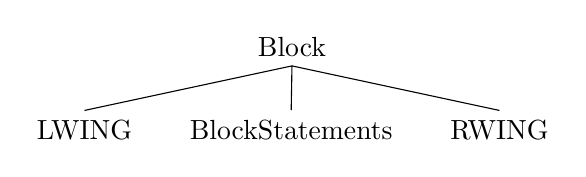
\begin{tikzpicture}[%
  sibling distance=.5cm,
  empty/.style={draw=none},
  tlabel/.style={font=\footnotesize\color{red!70!black}}]
\Tree  [.Block
         [.LWING ]
         [.BlockStatements ]
         [.RWING ]
       ]

\end{tikzpicture}
\caption{Ο κόμβος του AST που αφορά το Block}
\label{fig:block_node}
\end{figure}

Σκοπός του γεννήτορα είναι να διασχίσει τους διάφορους κόμβους του AST, δημιουργώντας παράλληλα τα αντίστοιχα στιγμιότυπα των εκφράσεων και των κανόνων.
Τελειώνοντας τη διάσχιση όλου του δέντρου, λοιπόν, θα έχει δημιουργήσει το στιγμιότυπο ολόκληρης της γραμματικής-στόχου (στο παράδειγμά μας, της Java).

Ενδεικτικά, ένας απλοποιημένος κώδικας για τη διάσχιση του κόμβου Block, το οποίο αποτελεί μία ακολουθία από εκφράσεις, θα ήταν όπως στο Σχήμα \ref{fig:factory_seq_example}.

\begin{figure}[h]
\setlength\partopsep{-\topsep}% adjusts vertical space after the listing
\begin{minted}[frame=lines,linenos,numbersep=5pt]{c++}
Expression* construct_sequence(TreeNode* node)
{
    if (node->children_num() > 1) {

        auto ce = new CompositeExpression('\b');

        for (auto child : node->get_children()) {
                Expression* e = traverse(child);
                ce->push_expr(e);
        }

        return ce;
    }
    else {
        return traverse(child);
    }
}
\end{minted}
\caption{Διάσχιση ακολουθίας και δημιουργία στιγμιοτύπων για τη γραμματική-στόχο}
\label{fig:factory_seq_example}
\end{figure}


Θεωρούμε ότι η traverse(child) επισκέπτεται το κάθε παιδί-κόμβο και δημιουργεί το αντίστοιχο μη τερματικό, επιστρέφοντάς το.
Οπότε, ο κώδικας λέει πως αν ο κόμβος έχει πάνω από ένα παιδί, τότε δημιούργησε ένα CompositeExpression ακολουθίας με όλα αυτά τα παιδιά ως μη τερματικά.
Αλλιώς, επίστρεψε απλά το μη τερματικό του ενός παιδιού.

Τελικά, για το παράδειγμά μας, τα στιγμιότυπα που θα γεννιούνταν θα ήταν όπως στο Σχήμα \ref{fig:objects_seq_example}. 

\begin{figure}[h]
\setlength\partopsep{-\topsep}% adjusts vertical space after the listing
\begin{minted}[frame=lines,linenos,numbersep=5pt]{c++}
NonTerminal parent("Block");
NonTerminal child1("LWING");
NonTerminal child2("BlockStatements");
NonTerminal child3("RWING");

// Block <- LWING BlockStatements RWING
CompositeExpression grammarExp('\b');
grammarExp.push_expr(&child1);
grammarExp.push_expr(&child2);
grammarExp.push_expr(&child3);
this->push_rule(&parent, &grammarExp);
\end{minted}
\caption{Στιγμιότυπα για τον πρώτο κανόνα της μετα-γραμματικής}
\label{fig:objects_seq_example}
\end{figure}

Διασχίζοντας όλο το AST, γεννιέται μία γραμματική Java, εκφρασμένη ως PEG.
Από αυτήν μπορύμε να φτιάξουμε τον αντίστοιχο Java packrat parser.
To τελευταίο βήμα για  τη διαδικασία του Σχήματος \ref{fig:peg_factory_pipeline}, είναι να δώσουμε ως είσοδο στον Java packrat parser ένα αρχείο Java.
Έτσι, παίρνουμε το AST για το .java αρχείο, οπότε ο στόχος μας επιτεύχθηκε.



\chapter{ Packrat Parsing με Ελαστικό Κυλιόμενο Παράθυρο}
\label{ch:elastic}

Όπως αναφέραμε, οι αναλυτές packrat, παρά την απλότητα και την γραμμική επίδοση (ως προς το μήκος της εισόδου) που προσφέρουν, έχουν το μειονέκτημα ότι καταναλώνουν πολύ χώρο για την αποθήκευση των ενδιάμεσων αποτελεσμάτων.
Αυτό αποτελεί αποθαρρυντικό παράγοντα για τη χρησιμοποίησή τους σε πολλές εφαρμογές.
Στην ενότητα αυτή περιγράφουμε μία ευριστική τεχνική για τη βελτίωση της κατανάλωσης μνήμης του packrat parser, χρησιμοποιώντας ένα \textit{κυλιόμενο παράθυρο (packrat parsing with elastic sliding window)} \cite{Kuramitsu2015a}.

\section{Εισαγωγή}

Η ιδέα πίσω από το packrat parsing με ελαστικό κυλιόμενο παράθυρο (ή πιο απλά elastic packrat parsing) βασίζεται στην έννοια του μήκους της μέγιστης οπισθαναχώρησης (longest backtrack length).
Ουσιαστικά, όταν προχωράει ο αναλυτής δεξιότερα ως προς την είσοδο, μπορεί να χρειαστεί να οπισθαναχωρήσει, όχι όμως αναγκαστικά μέχρι την αρχή της εισόδου, αλλά μέχρι ένα μικρότερο μήκος.
Έστω, ότι είχαμε έναν μικρότερο πίνακα υπομνηματισμού (παράθυρο) το οποίο "κυλάει" προς τα δεξιά ως προς την είσοδο και έχει επαρκές πλάτος ώστε να καλύπτει το μήκος της μέγιστης οπισθαναχώρησης. 
Τότε, ο πίνακας αυτός έχει τον απαραίτητο χώρο ώστε να αποθηκεύει όλα τα ενδιάμεσα αποτελέσματα, χωρίς να χρειαστεί οπισθαναχώρηση του αλγορίθμου.

Στην πράξη, βέβαια, είναι δύσκολο να ξέρουμε εκ των προτέρων πόση θα είναι η μέγιστη οπισθαναχώρηση.
Εναλλακτικά, επιλέγουμε ένα προσεγγιστικό μέγεθος για το παράθυρο από εμπειρικά δεδομένα και, αν χρειαστεί, το επεκτείνουμε κατά τη διάρκεια της συντακτικής ανάλυσης.

Όμως, η μέθοδος αυτή δεν περιορίζει μόνο τη χρήση κελιών ως προς τη διάσταση της εισόδου, αλλά και ως προς τη διάσταση των μη τερματικών συμβόλων.
Συγκεκριμένα, κατά την εκτέλεση της συντακτικής ανάλυσης μετριέται δυναμικά κατά πόσο κάθε μη τερματικό αξίζει να αποθηκεύεται στον πίνακα (παράθυρο) ή όχι.
Έτσι, ο χώρος που θα περισσέψει μπορεί να δοθεί ώστε να επεκταθεί το πλάτος του παραθύρου.
Εξ ού, και η "ελαστικότητα" του παραθύρου.

\section{Κυλιόμενο παράθυρο}

To παράθυρο πρακτικά είναι ένας buffer σταθερού μεγέθους, ο οποίος κυλάει προς τα δεξιά ως προς την είσοδο ώστε να περιλάβει τα νέα δεδομένα, ενώ τα παλιά δεδομένα απορρίπτονται από αυτόν. 
To Σχήμα \ref{fig:slide_window} απεικονίζει έναν buffer πλάτους 5 θέσεων πάνω από έναν πίνακα υπομνηματισμού.
Η δεξιότερη θέση του παραθύρου ταυτίζεται με το μέτωπο της συντακτικής ανάλυσης.

\begin{figure}[h]
	\centering
	\includegraphics[width=0.8\textwidth]{pics/slide_window} 
	\caption{Κυλιόμενο παράθυρο για τον πίνακα υπομνηματισμού \cite{Kuramitsu2015a}}
	\label{fig:slide_window}
\end{figure}

Αν το μέγεθος του παραθύρου δεν είναι επαρκώς μεγάλο, τότε θα "εκτοπιστεί" κάποιο χρήσιμο κελί του πίνακα υπομνηματισμού το οποίο περιέχει ένα ενδιάμεσο αποτέλεσμα που στο μέλλον θα χρειαστεί.
Αυτό σημαίνει ότι πρακτικά χάνεται η εγγύηση για γραμμικό χρόνο συντακτικής ανάλυσης, αφού το συγκεκριμένο κελί που χάθηκε θα πρέπει να υπολογιστεί ξανά, όπως θα έκανε ένας αναδρομικός αναλυτής με οπισθαναχώρηση.

Πόσο, όμως, πρέπει να έιναι το πλάτος του παραθύρου, ώστε να αποφευχθεί αυτή η δυσχέρεια?
Αυτή είναι μία δύσκολη ερώτηση. 
Θα μπορούσαμε να το κάνουμε όσο μεγάλη είναι και η είσοδος ώστε να μην ανησυχούμε για το αν θα χάσουμε κάποιο ενδιάμεσο αποτέλεσμα, όμως αυτό είναι ισοδύναμο με την αρχική έκδοση του packrat parsing.
Το άλλο άκρο θα ήταν το πλάτος να είναι $1$, που θα ισοδυναμούσε με έναν αναλυτή αναδρομικής κατάβασης με οπισθαναχώρηση.

Στο \cite{Kuramitsu2015a} παρουσιάζονται πειραματικές μετρήσεις για μία ποικιλία προγραμμάτων σε διάφορες γλώσσες, όπου φαίνεται πως οι πιο πολλές περιπτώσεις οπισθαναχώρησης συμβαίνουν σχετικά κοντά στο μέτωπο της συντακτικής ανάλυσης.
Συγκεκριμένα, ακόμα και ένα παράθυρο μήκους 16 bytes καταφέρνει να αποφύγει τον περιττό υπολογισμό κελιών στις περισσότερες περιπτώσεις οπισθαναχώρησης.

Το ξεκάθαρο πλεονέκτημα ενός παραθύρου είναι ότι διασφαλίζει ένα άνω φράγμα στη μνήμη που δεσμεύουμε στο σωρό.
Αν μάλιστα το μήκος του παραθύρου είναι επαρκές, τότε εξακολουθεί να ισχύει και η εγγύηση του γραμμικού χρόνου εκτέλεσης.
Ωστόσο, αν όχι, τότε υπάρχει ο κίνδυνος για ακόμα και εκθετικό χρόνο εκτέλεσης ως προς το μήκος της εισόδου, όπως θα έκανε ο αναλυτής αναδρομικής κατάβασης με οπισθαναχώρηση.

\section{Δυναμική απενεργοποίηση μη τερματικών συμβόλων}

Όπως αναφέραμε, στο elastic packrat parsing γίνεται προσπάθεια να περιοριστούν τα ενδιάμεσα αποτελέσματα που αποθηκεύονται, περιορίζοντας όχι μόνο το μήκος της εισόδου που καλύπτουμε, αλλά και τα μη τερματικά που εξυπηρετούμε.
Θα μπορούσαμε να την κάνουμε αυτή την ανάλυση στατικά, όμως η προσέγγιση που επιλέγεται είναι η δυναμική ανάλυση.

Συγκεκριμένα, ξεκινάμε θεωρώντας ότι όλα τα μη τερματικά είναι ενεργά, δηλαδή ότι αποθηκεύουμε ενδιάμεσα αποτελέσμα που τα αφορούν.
Δίνουμε σε όλα τα μη τερματικά έναν αριθμό ευκαιριών.
Στη συνέχεια, αν μετά από έναν συγκεκριμένο αριθμό κλήσεων για ένα μη τερματικό δούμε ότι τα ενδιάμεσα αποτελέσματα που το αφορούν δε χρησιμοποιήθηκαν ούτε μία φορά, το "απενεργοποιούμε" (Σχήμα \ref{fig:elastic_deactivate}).

\begin{figure}[h]
\setlength\partopsep{-\topsep}% adjusts vertical space after the listing
\begin{minted}[frame=lines,linenos,numbersep=5pt]{c++}
  ...
if (nt_elapsed[row] >= 0)  // μετράμε αντίστροφα όταν συναντάμε ένα μη τερματικό 
        nt_elapsed[row] = nt_elapsed[row] - 1;  // χωρίς να το χρησιμοποιήσουμε
  ...
if (nt_elapsed[row] == 0)  // αν έληξαν οι ευκαιρίες του
    if (!nt_utilized[row])  // και δε χρησιμοποιήθηκε ούτε μία φορά
        nt_activated[row] = false;  // το απενεργοποιούμε μόνιμα
  ...
\end{minted}
  \caption{Απενεργοποιήση μη τερματικού}
  \label{fig:elastic_deactivate}
\end{figure}

Δηλαδή, παύουμε να κρατάμε αποτελέσματα για αυτό, και όταν πρέπει να το αναλύσουμε, χρησιμοποιούμε απευθείας συντακτική ανάλυση αναδρομικής κατάβασης, χωρίς να εμπλακεί ο πίνακας ενδιάμεσων αποτελεσμάτων (Σχήμα \ref{fig:elastic_deactivated}).

\begin{figure}[h]
\setlength\partopsep{-\topsep}% adjusts vertical space after the listing
\begin{minted}[frame=lines,linenos,numbersep=5pt]{c++}
if (!nt_activated[row]) {
    Expression* e = peg.get_expr(&nt);
    return e->accept(*this);
}
\end{minted}
  \caption{Ένα απενεργοποιημένο μη τερματικό αναλύεται απευθείας χωρίς τη συμμετοχή του πίνακα 
  ενδιάμεσων αποτελεσμάτων.}
\label{fig:elastic_deactivated}
\end{figure}


Αν, ωστόσο, αξιοποιήσουμε έστω και ένα ενδιάμεσο αποτέλεσμα του μη τερματικού προτού απενεργοποιηθεί, το κρατάμε μόνιμα ενεργοποιημένο, όπως φαίνεται στο Σχήμα \ref{fig:elastic_keep_active}.


\begin{figure}[h]
\setlength\partopsep{-\topsep}% adjusts vertical space after the listing
\begin{minted}[frame=lines,linenos,numbersep=5pt]{c++}
  ...
case Result::success:  // έτοιμο αποτέλεσμα αποθηκευμένο 
{
    if (nt_elapsed[row] > 0) // αν δεν έχουν περάσει οι ευκαιρίες το κρατάμε μόνιμα ενεργό
        nt_utilized[row] = true;
    pos = cur_cell->pos();
    return true;
}
case Result::fail:  // έτοιμο αποτέλεσμα αποθηκευμένο 
{
    if (nt_elapsed[row] > 0) // αν δεν έχουν περάσει οι ευκαιρίες το κρατάμε μόνιμα ενεργό
        nt_utilized[row] = true;
    return false;
}
  ...
\end{minted}
  \caption{Aξιοποιήση ενός κελιού για ένα μη τερματικό προτού λήξουν οι ευκαιρίες και μόνιμη ενεργοποίησή του}
\label{fig:elastic_keep_active}
\end{figure}

Το ποιο θα είναι αυτό το "κατώφλι", δηλαδή ο αριθμός κλήσεων στο μη τερματικό που δεν αξιοποιεί ούτε ένα ενδιάμεσο αποτέλεσμα, είναι μια παράμετρος που πρέπει να μετρήσουμε.

\section{Elastic Packrat Parsing}

Το elastic packrat parsing είναι μία μέθοδος που συνδυάζει τόσο το κυλιόμενο παράθυρο, όσο και τη δυναμική απενεργοποίηση μη τερματικών.

To Σχήμα \ref{fig:elastic_slide_window} απεικονίζει την ιδέα.

\begin{figure}[h]
	\centering
	\includegraphics[width=0.8\textwidth]{pics/elastic_slide_window} 
	\caption{Ελαστικό κυλιόμενο παράθυρο \cite{Kuramitsu2015a}}
	\label{fig:elastic_slide_window}
\end{figure}

Για την υλοποίηση, χρησιμοποιούμε έναν μονοδιάστατο πίνακα $W*N$, όπου $W$ είναι το πλάτος του παραθύρου και $N$ ο αριθμός των ενεργών μη τερματικών.
Οπότε, ένα ζεύγος $(position, non terminal)$ αντιστοιχεί σε μία θέση στον μονοδιάστατο πίνακα.
Ακολούθως, χρησιμοποιούμε έναν δείκτη κατακερματισμού (hasing-based index) για να εντοπίσουμε σε ποιο σημείο του μονοδιάστατου πίνακα θα αποθηκευτεί το ενδιάμεσο αποτέλεσμα, όπως στο Σχήμα \ref{fig:elastic_1}.
Φτιάχνουμε, αρχικά, ένα κλειδί μέσω της θέσης και του μη τερματικού, το οποίο μετά το ελαττώνουμε μέσω του modulo ($W*N$).

\begin{figure}[h]
\setlength\partopsep{-\topsep}% adjusts vertical space after the listing
\begin{minted}[frame=lines,linenos,numbersep=5pt]{c++}
    long int key = (pos << shift) | row;
    unsigned int index = hash(key) % (w * n);
    ...
    ElasticCell* cur_cell = &elastic_cells[index];    // πάρε το αντίστοιχο κελί
    cur_cell->set_key(key);        // θέσε το κλειδί στο αντίστοιχο κελί
\end{minted}
\caption{Δημιουργία κλειδιού και δείκτη}
\label{fig:elastic_1}
\end{figure}

Το πλεονέκτημα είναι ότι όταν απενεργοποιούμε ένα μη τερματικό, ο χώρος του στον πίνακα μπορεί να αξιοποιηθεί από άλλα μη τερματικά, διευρύνοντας ουσιαστικά το παράθυρο, όπως δείχνει το Σχήμα \ref{fig:elastic_slide_window}. 
Αυτή είναι και η ουσία της ελαστικότητας της μεθόδου. 
Στην ακραία περίπτωση που μόνο ένα μη τερματικό μείνει ενεργοποιημένο, τότε το παράθυρο έχει πρακτικά μέγεθος ίσο με $W*N$ και τη μορφή μίας γραμμής.

Το μειονέκτημα του hashing-based index είναι πως μπορεί να υπάρχουν συγκρούσεις (collisions) μεταξύ διαφορετικών κλειδιών, που όμως αντιστοιχίζονται στο ίδιο index.
Αυτό αίρει την αυστηρότητα στην αποθήκευση ενδιάμεσων αποτελεσμάτων, αλλά τα οφέλη μίας τέτοιας απλής πρακτικής είναι μεγαλύτερα στη συνήθη περίπτωση.

Τέλος, η τεχνική αυτή δεν περιλαμβάνει ρητή κύλιση του παραθύρου, για πιο απλή υλοποίηση.
Αντίθετα, η κύλιση προς τα δεξιά επιτυγχάνεται έμμεσα, καθώς τα νέα κλειδιά που αποθηκεύονται και αντιστοιχούν σε δεξιότερα σημεία της εισόδου, αντικαθιστούν τα παλιά.
Αυτό προσεγγίζει την κύλιση, η οποία θα κόστιζε πολύ περισσότερο σε υλοποιήση για να γίνεται επ'ακριβώς.

Στο Κεφάλαιο \ref{ch:packrat} αναφέραμε ότι ο αλγόριθμος packrat καταναλώνει χώρο $O(NT * n)$, όπου $NT$ ο αριθμός των μη τερματικών της εκάστοτε γραμματικής, και $n$ το μήκος της εισόδου. 
Τώρα, φαίνεται ότι ο απαιτούμενος χώρος εκτέλεσης γίνεται $O(NT * W)$, όπου $W$ το μήκος του παραθύρου, το οποίο είναι σταθερό.
Δηλαδή, πλέον, ο χώρος εκτέλεσης δεν είναι γραμμικός, αλλά σταθερός ως προς το μήκος της εισόδου, κάτι που αποτελεί μεγάλο πλεονέκτημα σε σχέση με τον κλασικό αλγόριθμο.


\chapter{ Parallel Packrat Parsing }
\label{ch:parallel}

Η βασική συνεισφορά που θέλουμε να κάνουμε στα πλαίσια της διπλωματικής, είναι να τροποποιήσουμε τη σειριακή έκδοση του packrat parser, ώστε να μπορεί να τρέξει αποδοτικότερα σε ένα πολυπύρηνο σύστημα.
Επιπλέον, θα δοκιμάσουμε τα παραλληλοποιήσουμε όχι μόνο την κλασική έκδοση του packrat, αλλά και παραλλαγών της.

To πρόβλημα εύρεσης παραλληλισμού δεν είναι καθόλου τετριμμένο εν γένει. 
Ειδικά στην περίπτωση μας, θα πρέπει να εξετάσουμε διάφορα κομμάτια του αλγορίθμου που μπορούν να μοιραστούν μεταξύ των νημάτων, καθώς και πώς τα νήματα αυτά θα προσπελάσουν τη δομή δεδομένων με τα ενδιάμεσα αποτελέσματα.
Εδώ, πρέπει να προσέξουμε ιδιαιτέρως δύο σημεία:

\begin{description}[font=$\bullet$\scshape\bfseries]
	\item Η πρόσβαση σε κάθε κελί της δομής δεδομένων πρέπει να γίνεται με \textit{αμοιβαίο αποκλεισμό (mutual exlusion)} μεταξύ των νημάτων.
	\item Θέλουμε η \textit{αναμονή (waiting)} των νημάτων να είναι όσο το δυνατόν μικρότερη.
\end{description}

Θα ξεκινήσουμε πρώτα με τον αλγόριθμο δυναμικού προγραμματισμού για το packrat parsing (DP packrat).
Ακολούθως, θα επικεντρωθούμε στον αλγόριθμο με υπομνηματισμό.
Θα δούμε τί έχει δοκιμαστεί ως τώρα από την επιστημονική κοινότητα, ενώ θα επιχειρήσουμε και δικές μας προσεγγίσεις.

\section{Παράλληλος DP packrat}



\chapter{Πειραματικά Αποτελέσματα}
\label{ch:results}

\begin{figure}
    \begin{tikzpicture}
    \begin{axis}
    [   view={-45}{60},
    xmin=0,xmax=10,
    ymin=0,ymax=10,
    zmin=0, zmax=10,
    ]
    \addplot3[scatter, only marks] file{./a.dat};
    \end{axis}

    \end{tikzpicture}
\end{figure}


\chapter{ Συμπεράσματα }
\label{ch:conclusions}

Οι Parsing Expression Grammars αποτελούν διαισθητικά ένα κατάλληλο εργαλείο προσδιορισμού γραμματικών, ιδιαίτερα αν συγκριθούν με τις γραμματικές χωρίς συμφραζόμενα. 
Αρχικά, ο σχεδιαστής της γραμματικής είναι ευκολότερο να σκέφτεται πώς αναλύεται μία δοσμένη συμβολοσειρά στα συστατικά της, σε σχέση με το πώς θα γεννηθεί η συμβολοσειρά μέσα από τους κανόνες της γραμματικής (στο πνεύμα των Context Free γραμματικών).
Επιπλέον, ο ίδιος ο ορισμός των PEGs ορίζει απευθείας και τον αντίστοιχο συντακτικό αναλυτή της γραμματικής αυτής.

Ένας γεννήτορας συντακτικών αναλυτών είναι ένα βολικό εργαλείο για να φτιάχνουμε αυτόματα αναλυτές για μία γραμματική PEG που έχουμε ορίσει τυπικά.
Ο γεννήτορας παίρνει ως είσοδο μία τυπική περιγραφή της PEG και δίνει ως έξοδο ένα στιγμιότυπο της γραμματικής αυτής που μπορεί να αναλύσει ένας packrat parser.
Ο γεννήτορας πρακτικά δημιουργεί γραμματικές αλλά, όπως είπαμε, η κατασκευή μίας PEG συνεπάγεται και την κατασκευή του αντίστοιχου συντακτικού αναλυτή.
Επομένως, ο γεννήτορας κατασκευάζει συντακτικούς αναλυτές.

Ιδιαίτερα, λοιπόν, αν ο προκύπτων συντακτικός αναλυτής είναι και αποδοτικός στο χρόνο και στο χώρο, ένα τέτοιο εργαλείο θα ήταν βολικό για έναν προγραμματισή ο οποίος πειραματίζεται με μία δική του γραμματική για κάποιον ειδικό σκοπό.
Διότι, έχει τη δυνατότητα να ορίσει και να αλλάζει εύκολα τον ορισμό της γραμματικής του, αλλά και να παίρνει έναν γρήγορο συντακτικό αναλυτή για τις εφαρμογές του.

Από το προηγούμενο κεφάλαιο φαίνεται μάλλον ότι το packrat parsing με ελαστικό κυλιόμενο παράθυρο αποτελεί την καλύτερη βελτίωση του packrat, καθώς χρειάζεται αισθητά λιγότερο χρόνο εκτέλεσης, αλλά και σταθερή μνήμη, εξοβελίζοντας ένα κυρίαρχο μειονέκτημα του κλασικού αλγορίμου.




\selectlanguage{greek}

%%%  Bibliography

% You shouldn't want to include all the contents of thesis.bib
% in your bibliography (do you?)
\nocite{*}

\bibliographystyle{softlab-thesis}
\bibliography{thesis}


%%%  Appendices

\backmatter

\appendix

\chapter{Μία PEG περιγράφει τυπικά την ίδια τη σύνταξη της}

\begin{Verbatim}
# Hierarchical syntax

Grammar    <- Spacing Definition+ EndOfFile                     # Type 0
Definition <- Identifier LEFTARROW Expression                   # Type 1
Expression <- Sequence (SLASH Sequence)*                        # Type 2
Sequence   <- Prefix*                                           # Type 3
Prefix     <- (AND / NOT)? Suffix                               # Type 4
Suffix     <- Primary (QUESTION / STAR / PLUS)?                 # Type 5
Primary    <- Identifier !LEFTARROW                             # Type 6
            / OPEN Expression CLOSE
            / Literal / DOT

# Lexical syntax

Identifier <- IdentifierStart IdentifierRest* Spacing
IdentifierStart <- 'a' / 'b' / 'c' / 'd' / 'e' / 'f' / 'g' / 'h' /
		   'i' / 'j' / 'k' / 'l' / 'm' / 'n' / 'o' / 'p' /
		   'q' / 'r' / 's' / 't' / 'u' / 'v' / 'w' / 'x' / 'y' / 'z' /
		   ᾽A' / 'B' / 'C' / 'D' / 'E' / 'F' / 'G' / 'H' /
		   'I' / 'J' / 'K' / 'L' / 'M' / 'N' / 'O' / 'P' /
		   'Q' / 'R' / 'S' / 'T' / 'U' / 'V' / 'W' / 'X' / 'Y' / 'Z' / '_'

IdentifierRest <- 'a' / 'b' / 'c' / 'd' / 'e' / 'f' / 'g' / 'h' /
		  'i' / 'j' / 'k' / 'l' / 'm' / 'n' / 'o' / 'p' /
		  'q' / 'r' / 's' / 't' / 'u' / 'v' / 'w' / 'x' / 'y' / 'z' /
		  'A' / 'B' / 'C' / 'D' / 'E' / 'F' / 'G' / 'H' /
		  'I' / 'J' / 'K' / 'L' / 'M' / 'N' / 'O' / 'P' /
		  'Q' / 'R' / 'S' / 'T' / 'U' / 'V' / 'W' / 'X' / 'Y' / 'Z' / '_' /
		  '0' / '1' / '2' / '3' / '4' / '5' / '6' / '7' / '8' / '9'

Literal    <- "'" (!"'" Character)* "'" Spacing                 # Type 8
            / '"' (!'"' Character)* '"' Spacing

Character  <- ('\\' ('n' / 'r' / 't' / '\\' / "'" / '"' / UnicodeEscape)) / (!'\\' .)

UnicodeEscape <- 'u' UnicodeElement UnicodeElement UnicodeElement UnicodeElement

UnicodeElement <- '0' / '1' / '2'/ '3' / '4' / '5' / '6' / '7' / '8' / '9' /
		  'A' / 'B' / 'C' / 'D'/ 'E' / 'F' / 'a' / 'b' / 'c' / 'd'/ 'e' / 'f'


LEFTARROW  <- '<-' Spacing                                      # Type 10
SLASH      <- '/' Spacing                                       # Type 11
AND        <- '&' Spacing                                       # Type 12
NOT        <- '!' Spacing                                       # Type 13
QUESTION   <- '?' Spacing                                       # Type 14
STAR       <- '*' Spacing                                       # Type 15
PLUS       <- '+' Spacing                                       # Type 16
OPEN       <- '(' Spacing                                       # Type 17
CLOSE      <- ')' Spacing                                       # Type 18
DOT        <- '.' Spacing                                       # Type 19
Spacing    <- (Space / Comment)*                                # Type 20
Comment    <- '#' (!EndOfLine .)* EndOfLine                     # Type 21
Space      <- ' ' / '\t' / EndOfLine                            # Type 22
EndOfLine  <- '\r\n' / '\n' / '\r'                              # Type 23
EndOfFile  <- !.                                                # Type 24
\end{Verbatim}

%%%  End of document

\end{document}
